\clearpage

\section{Results and discussion \label{sec:conclusion}}

Our 1D shape analyses using the mass variables $M_\Delta^R$, $M_{CT\perp}$, and $M_{T2}$ allow
a fair and realistic comparison of their discriminating power.
We begin by plotting the expected exclusion sensitivity for left-handed selectrons or charginos decaying to neutralinos, as a function of selectron/chargino and neutralino masses, assuming 20~fb$^{-1}$ of data from a single experiment at the 8~TeV LHC. Charginos are assumed to decay into $W$ bosons and an invisible neutralino, followed by Standard Model decays of the $W$ bosons into leptons. Results for left-handed smuons would be similar to those for the selectron, but we assume only a single species of slepton for our analysis. In Figures~\ref{fig:results_slepton_2D_compare} and \ref{fig:results_chargino_2D_compare}, we show the expected exclusion reach (at 95\% confidence level) of the ATLAS $M_{T2}$ and CMS $M_{CT\perp}$ analyses compared to the new technique using $M_\Delta^R$. In making the comparisions we use the same sets of ATLAS or CMS cuts as the existing experimental searches, which are not optimized for our analysis. 
Even with this disadvantage the expected exclusion limits using the super-razor variable $M_\Delta^R$ outperform the $M_{CT\perp}$ searches in terms of both absolute slepton or chargino mass and near the degenerate limit (when the mass of the parent is close to the mass of the invisible daughter). We show selected slices of these analyses in Figure~\ref{fig:results_1D_compare}, fixing either the selectron or neutralino mass, and varying the other. This allows a more direct comparison of our new variable $M_\Delta^R$ to the alternative techniques. Again the sensitivity using $M_\Delta^R$ outperforms
that obtained from $M_{CT\perp}$. For these 1D analyses the performance using $M_{T2}$ is only
slightly worse than that obtained with $M_\Delta^R$.

\begin{figure}[ht]
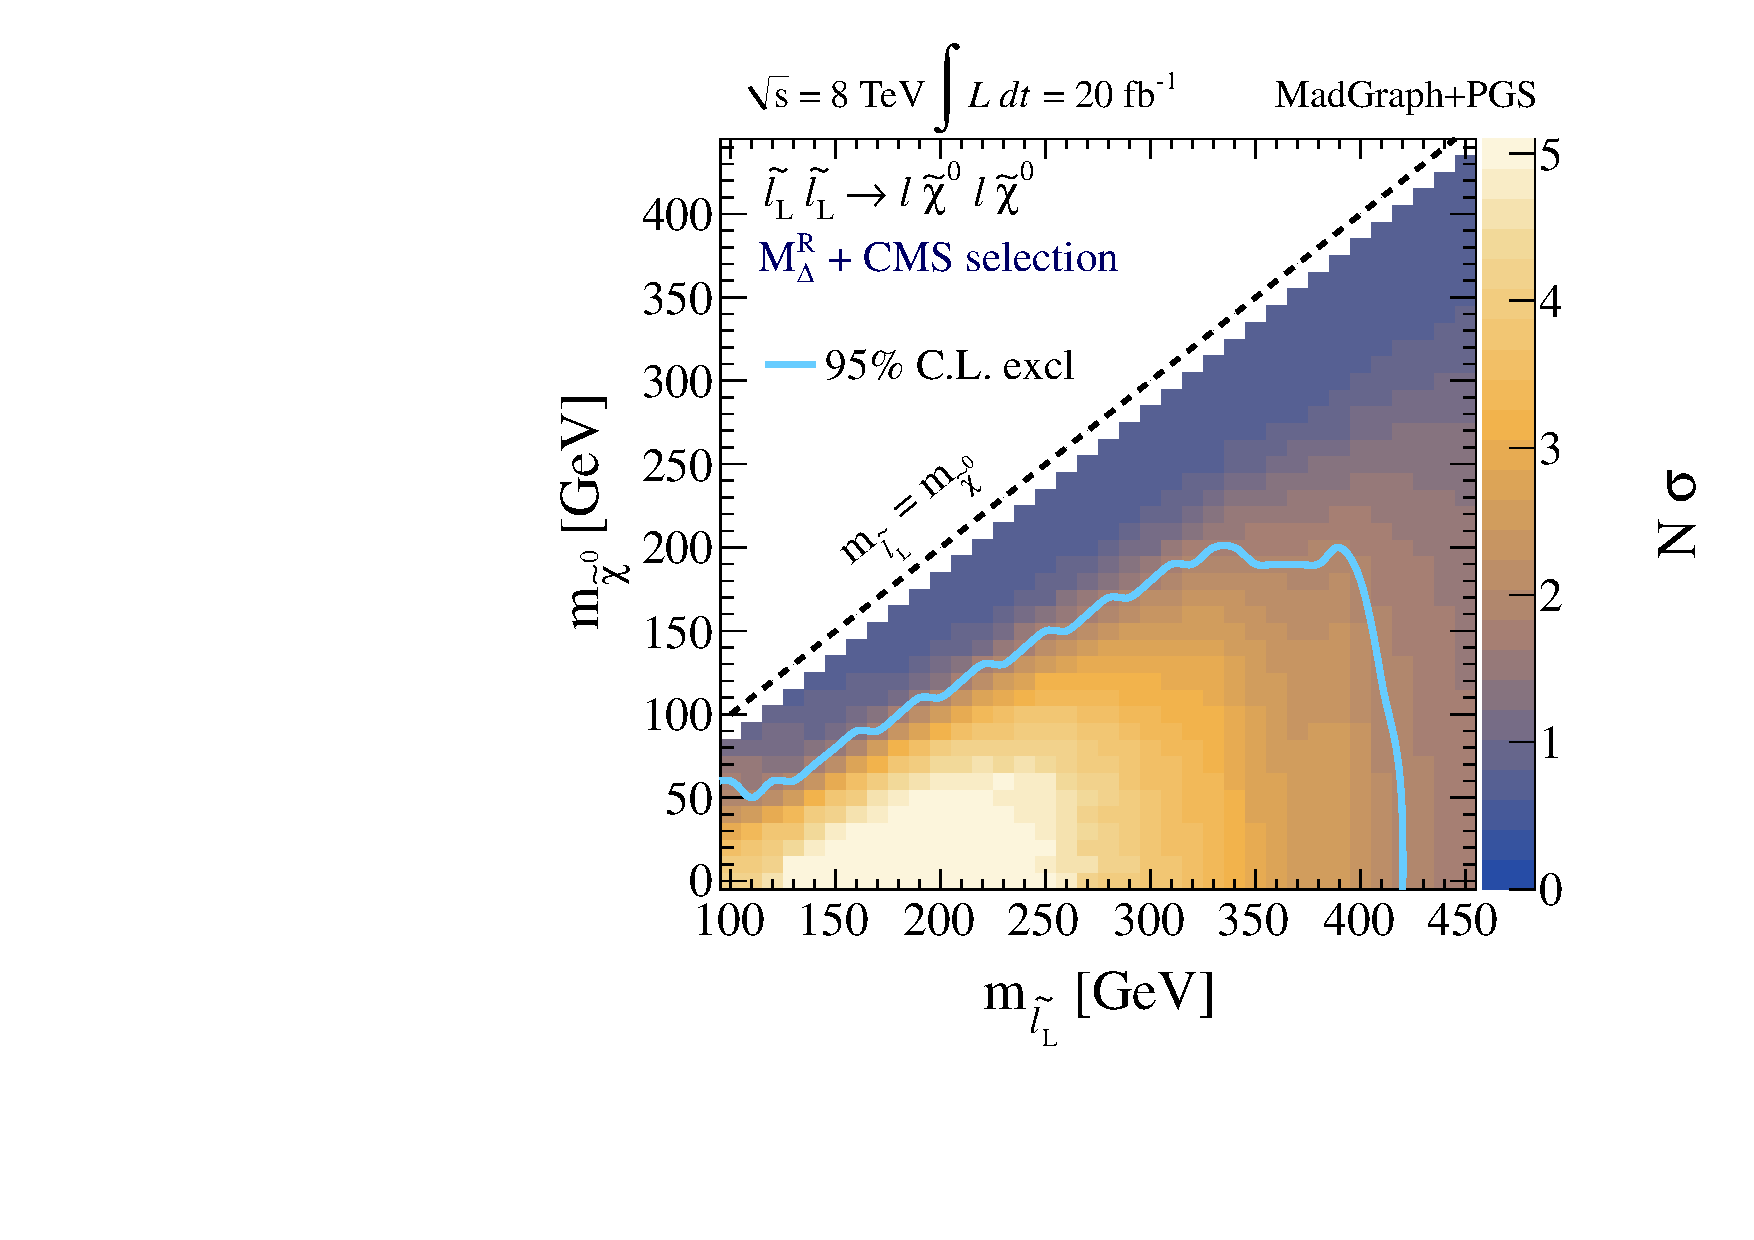
\includegraphics[width=0.4\columnwidth]{fig/sectionV/LIMIT2D_selectronL_CMS_Mdelta.pdf}
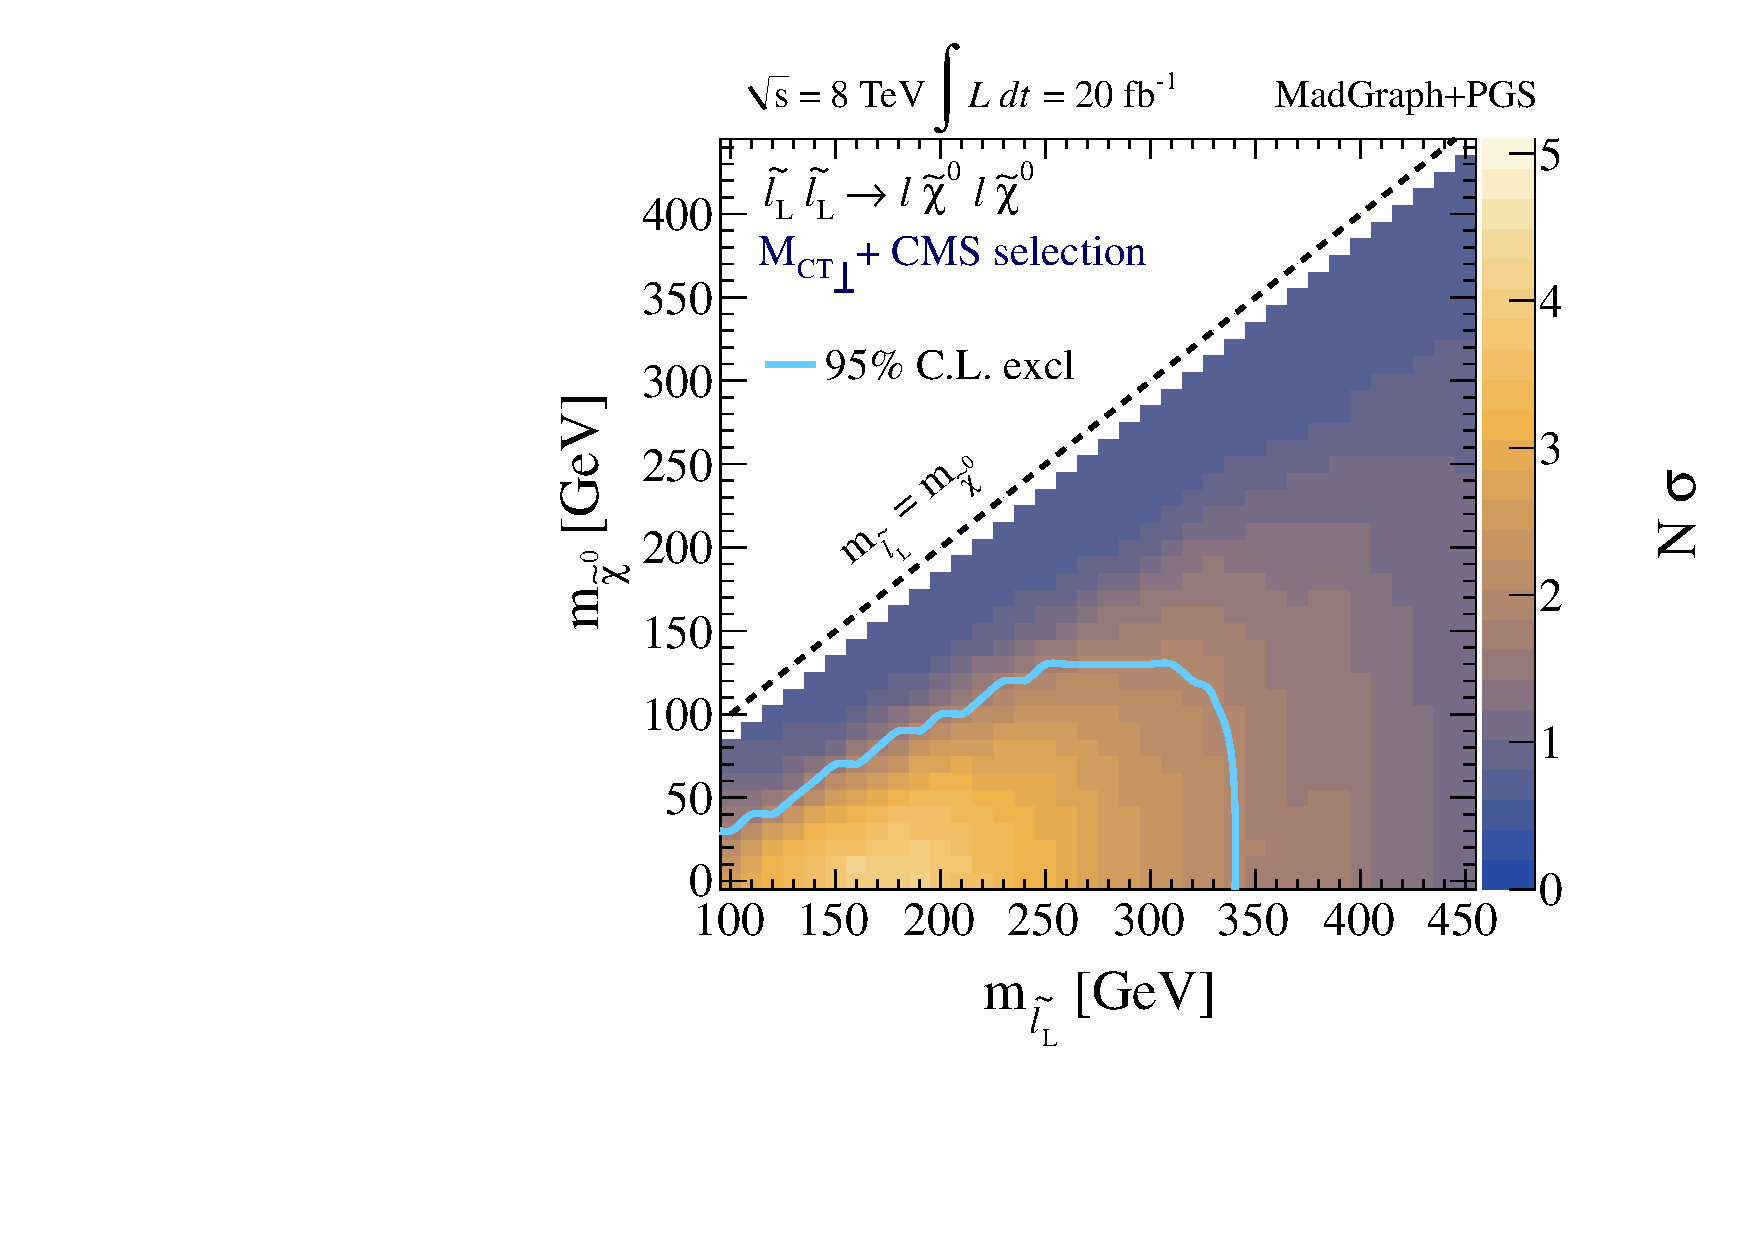
\includegraphics[width=0.4\columnwidth]{fig/sectionV/LIMIT2D_selectronL_CMS_MCTperp.pdf}
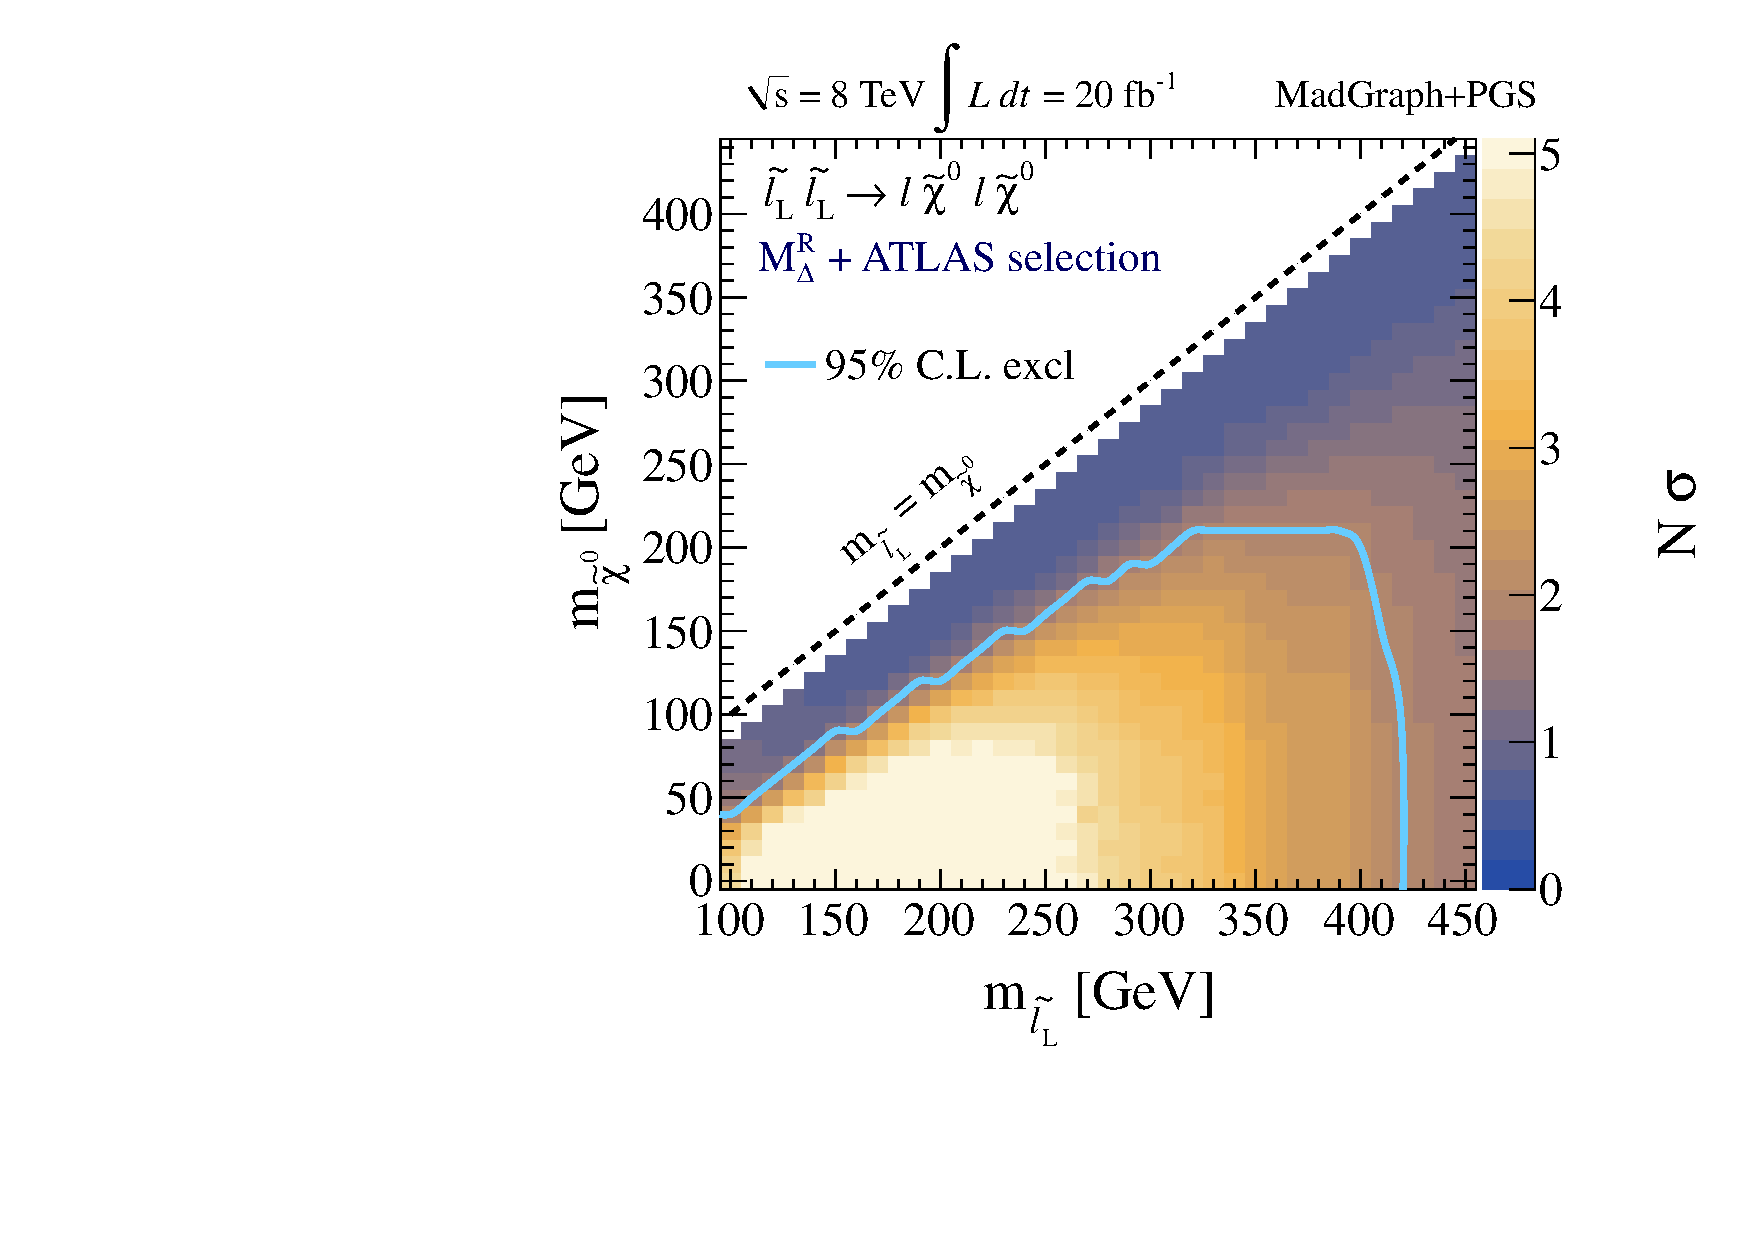
\includegraphics[width=0.4\columnwidth]{fig/sectionV/LIMIT2D_selectronL_ATLAS_Mdelta.pdf}
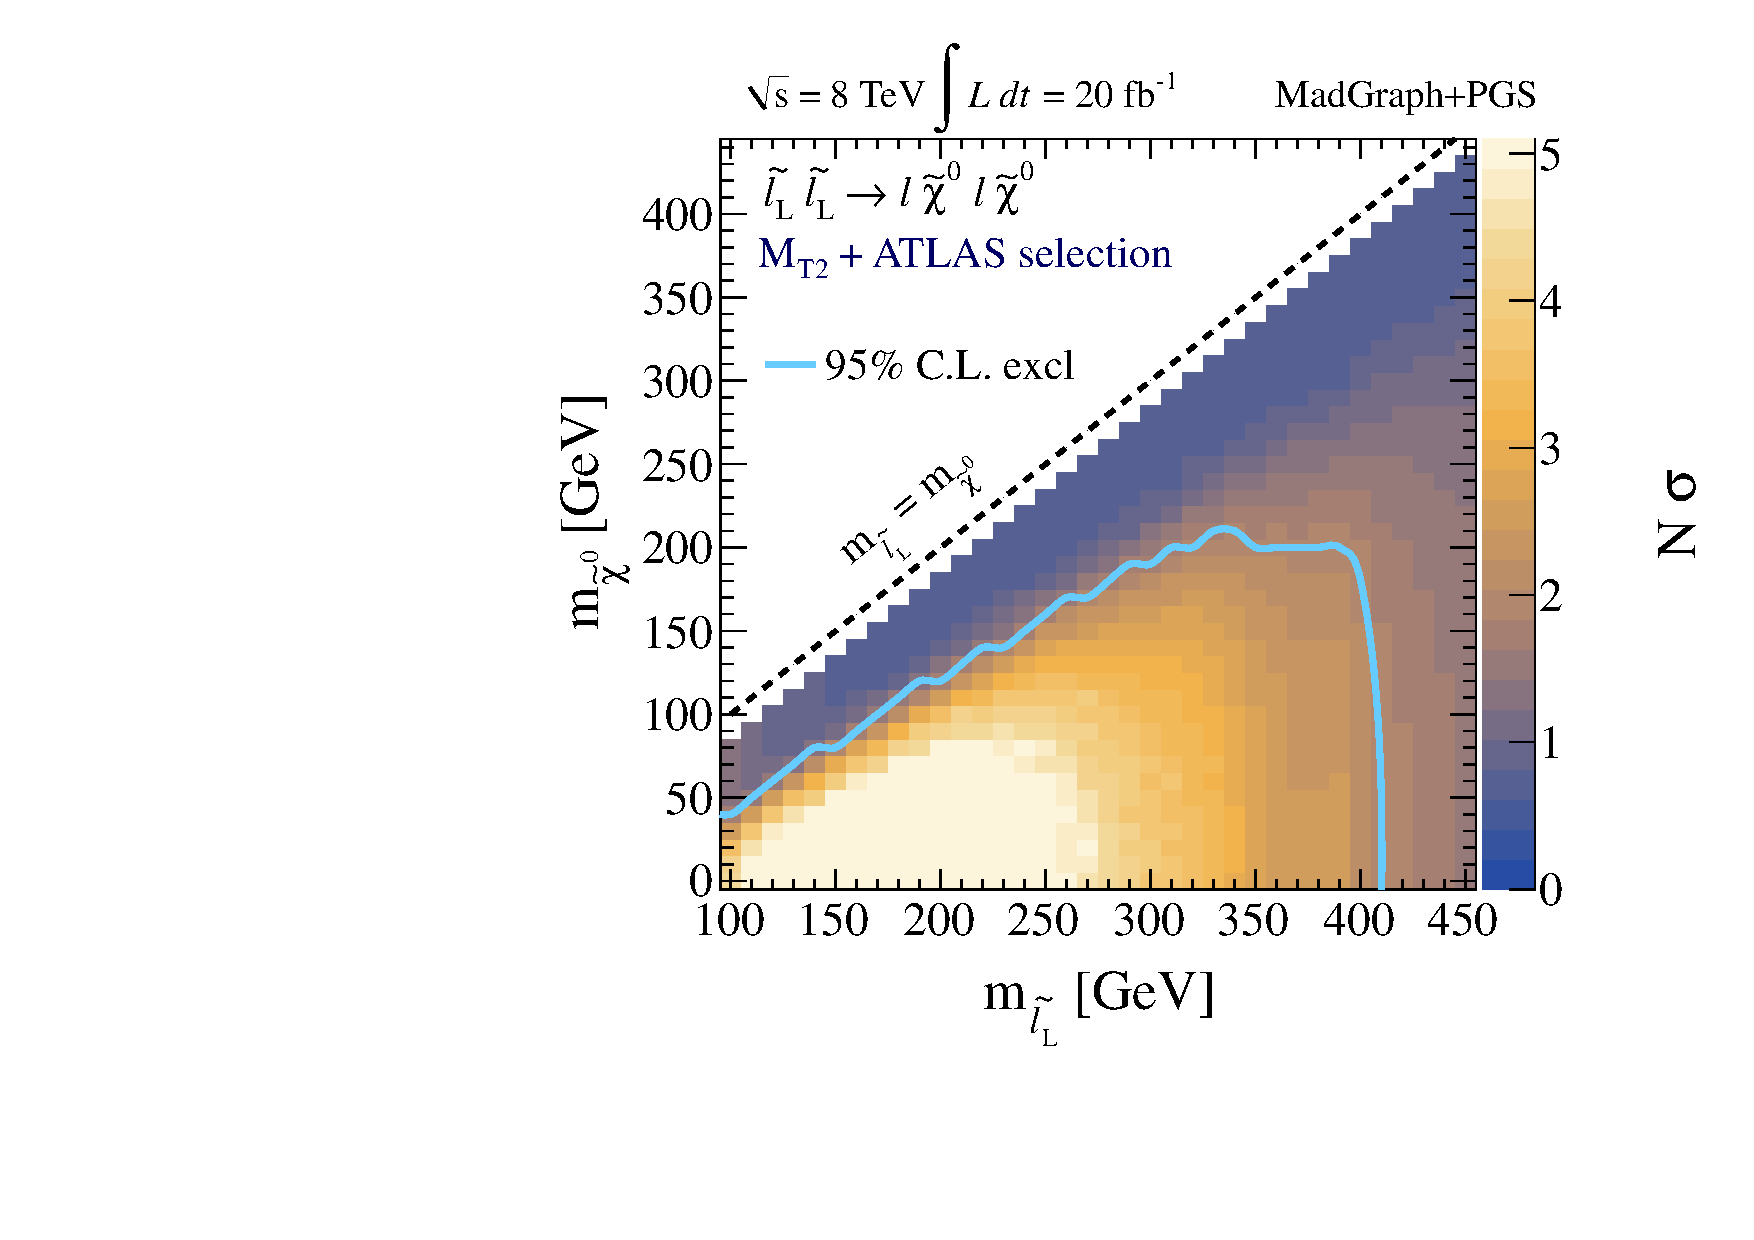
\includegraphics[width=0.4\columnwidth]{fig/sectionV/LIMIT2D_selectronL_ATLAS_MT2.pdf}
\caption{Expected exclusion limits (in units of $\sigma$) for left-handed selectrons decaying to leptons and neutralinos using 20~fb$^{-1}$ of 8 TeV data, as a function of both selectron and neutralino masses. Expected limits are shown for our 1D $M_\Delta^R$ analysis using CMS (upper left) and ATLAS (lower left) selection cuts, and directly compared to our expected exclusions using our simulated CMS $M_{CT\perp}$ (upper right) and ATLAS $M_{T2}$ (lower right) analyses. \label{fig:results_slepton_2D_compare}}
\end{figure}

\begin{figure}[ht]
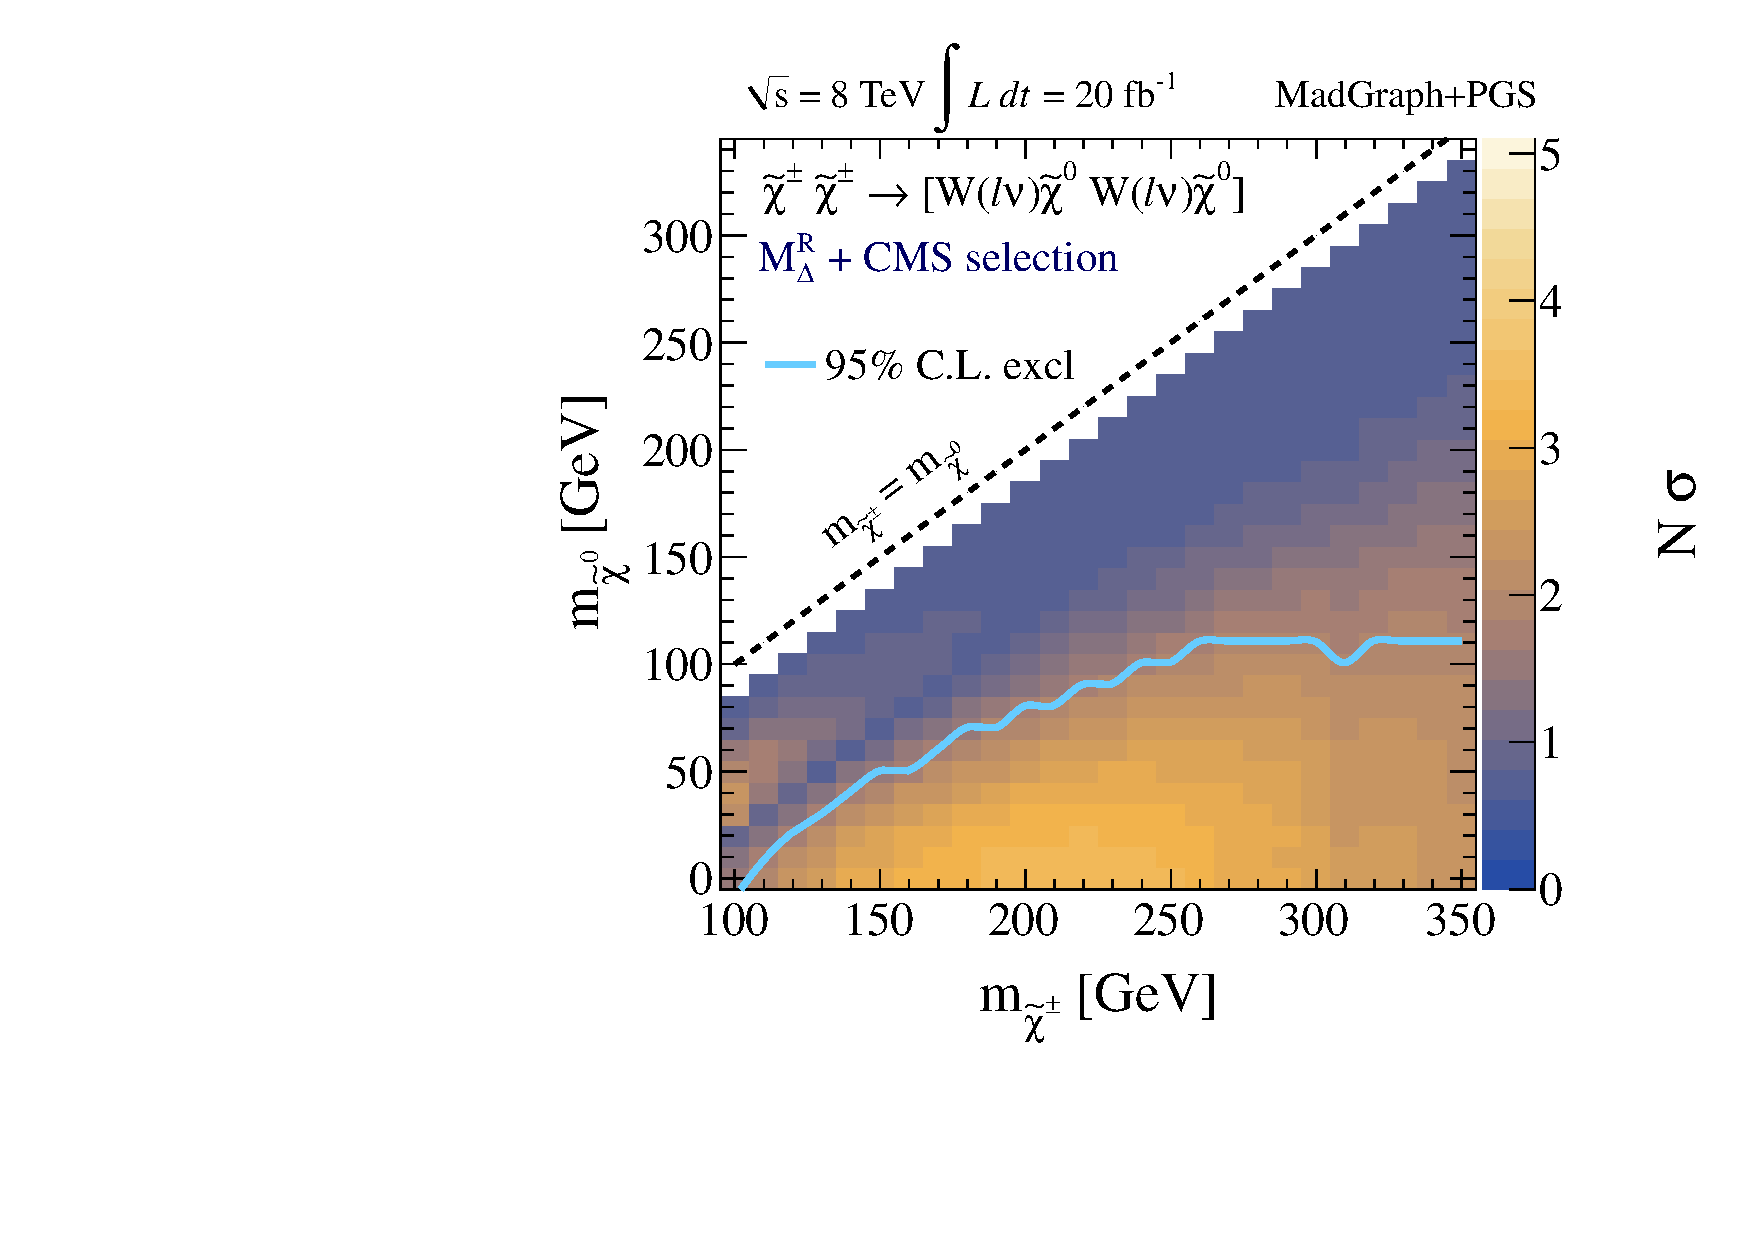
\includegraphics[width=0.4\columnwidth]{fig/sectionV/LIMIT2D_chargino_CMS_Mdelta.pdf}
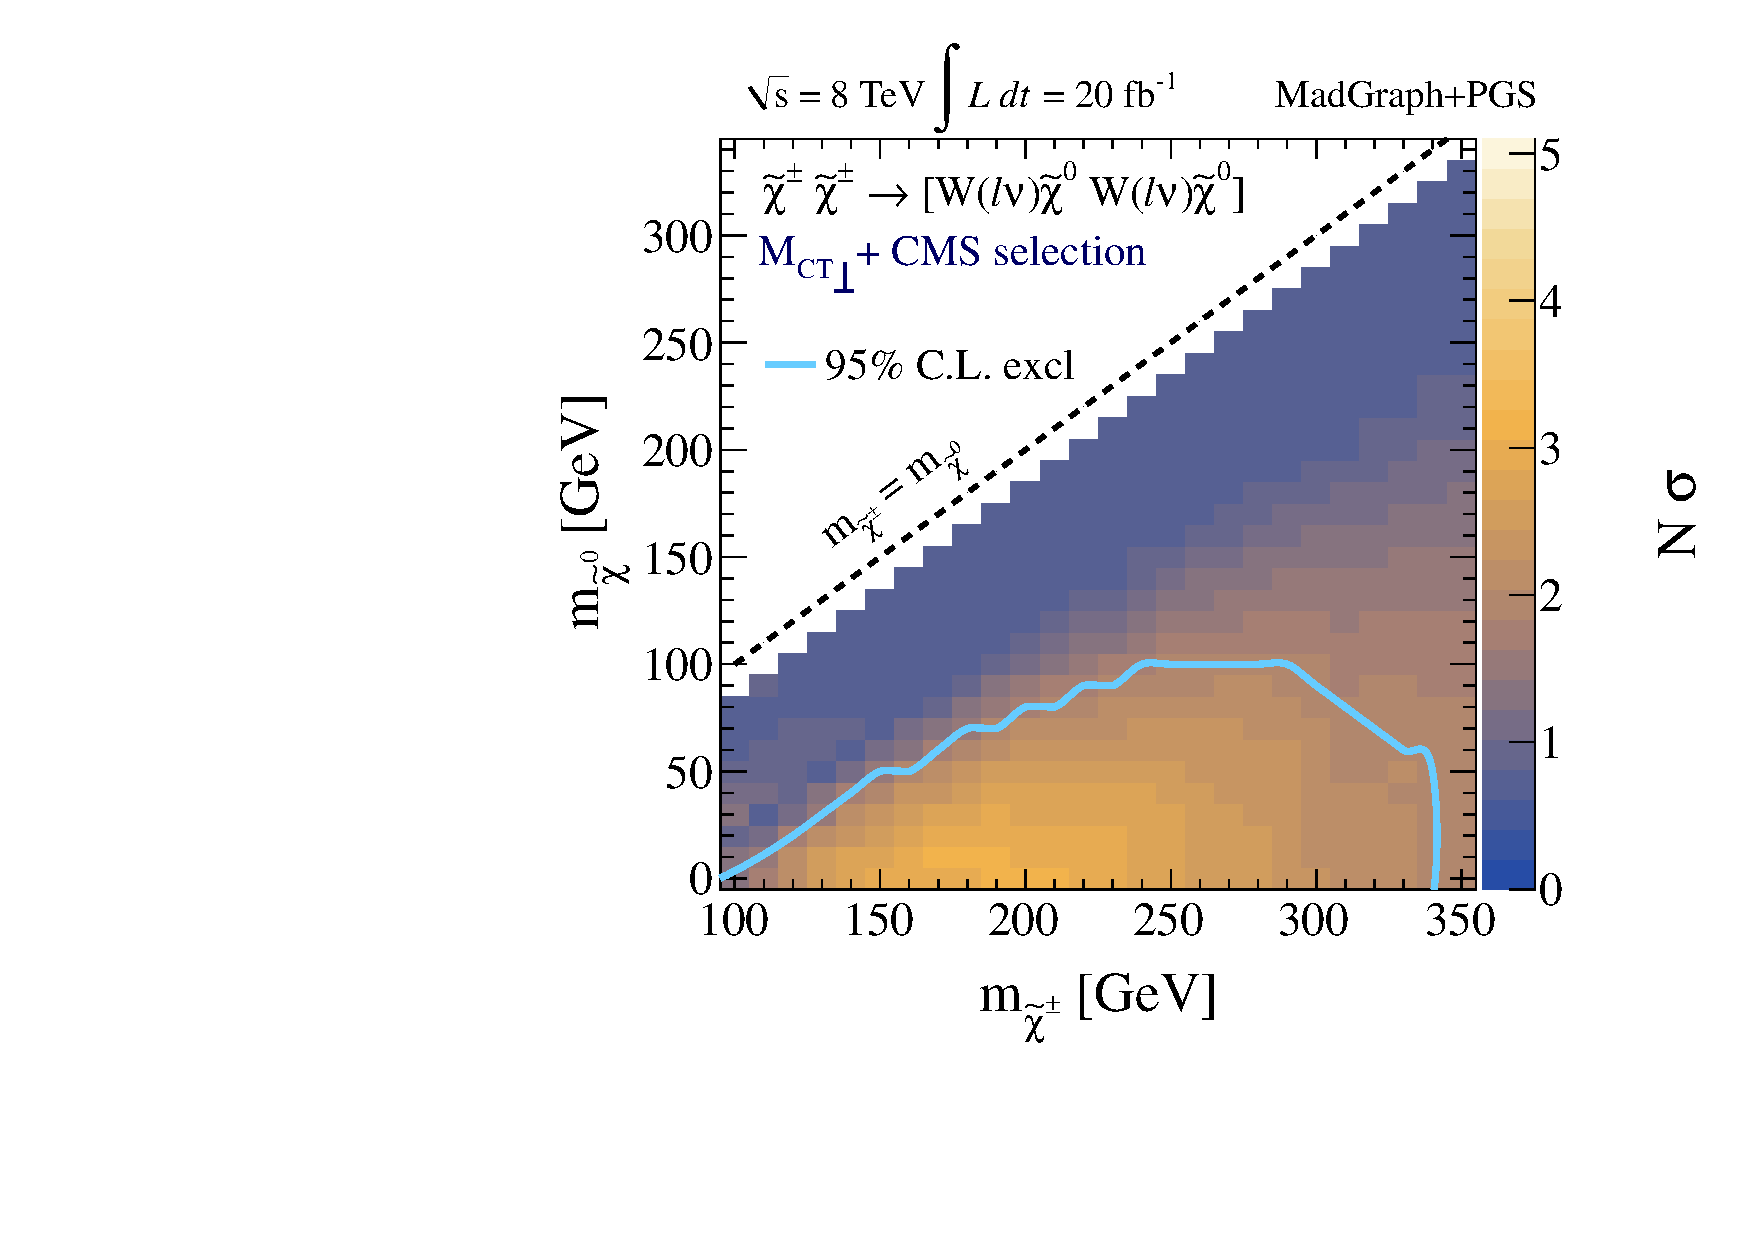
\includegraphics[width=0.4\columnwidth]{fig/sectionV/LIMIT2D_chargino_CMS_MCTperp.pdf}
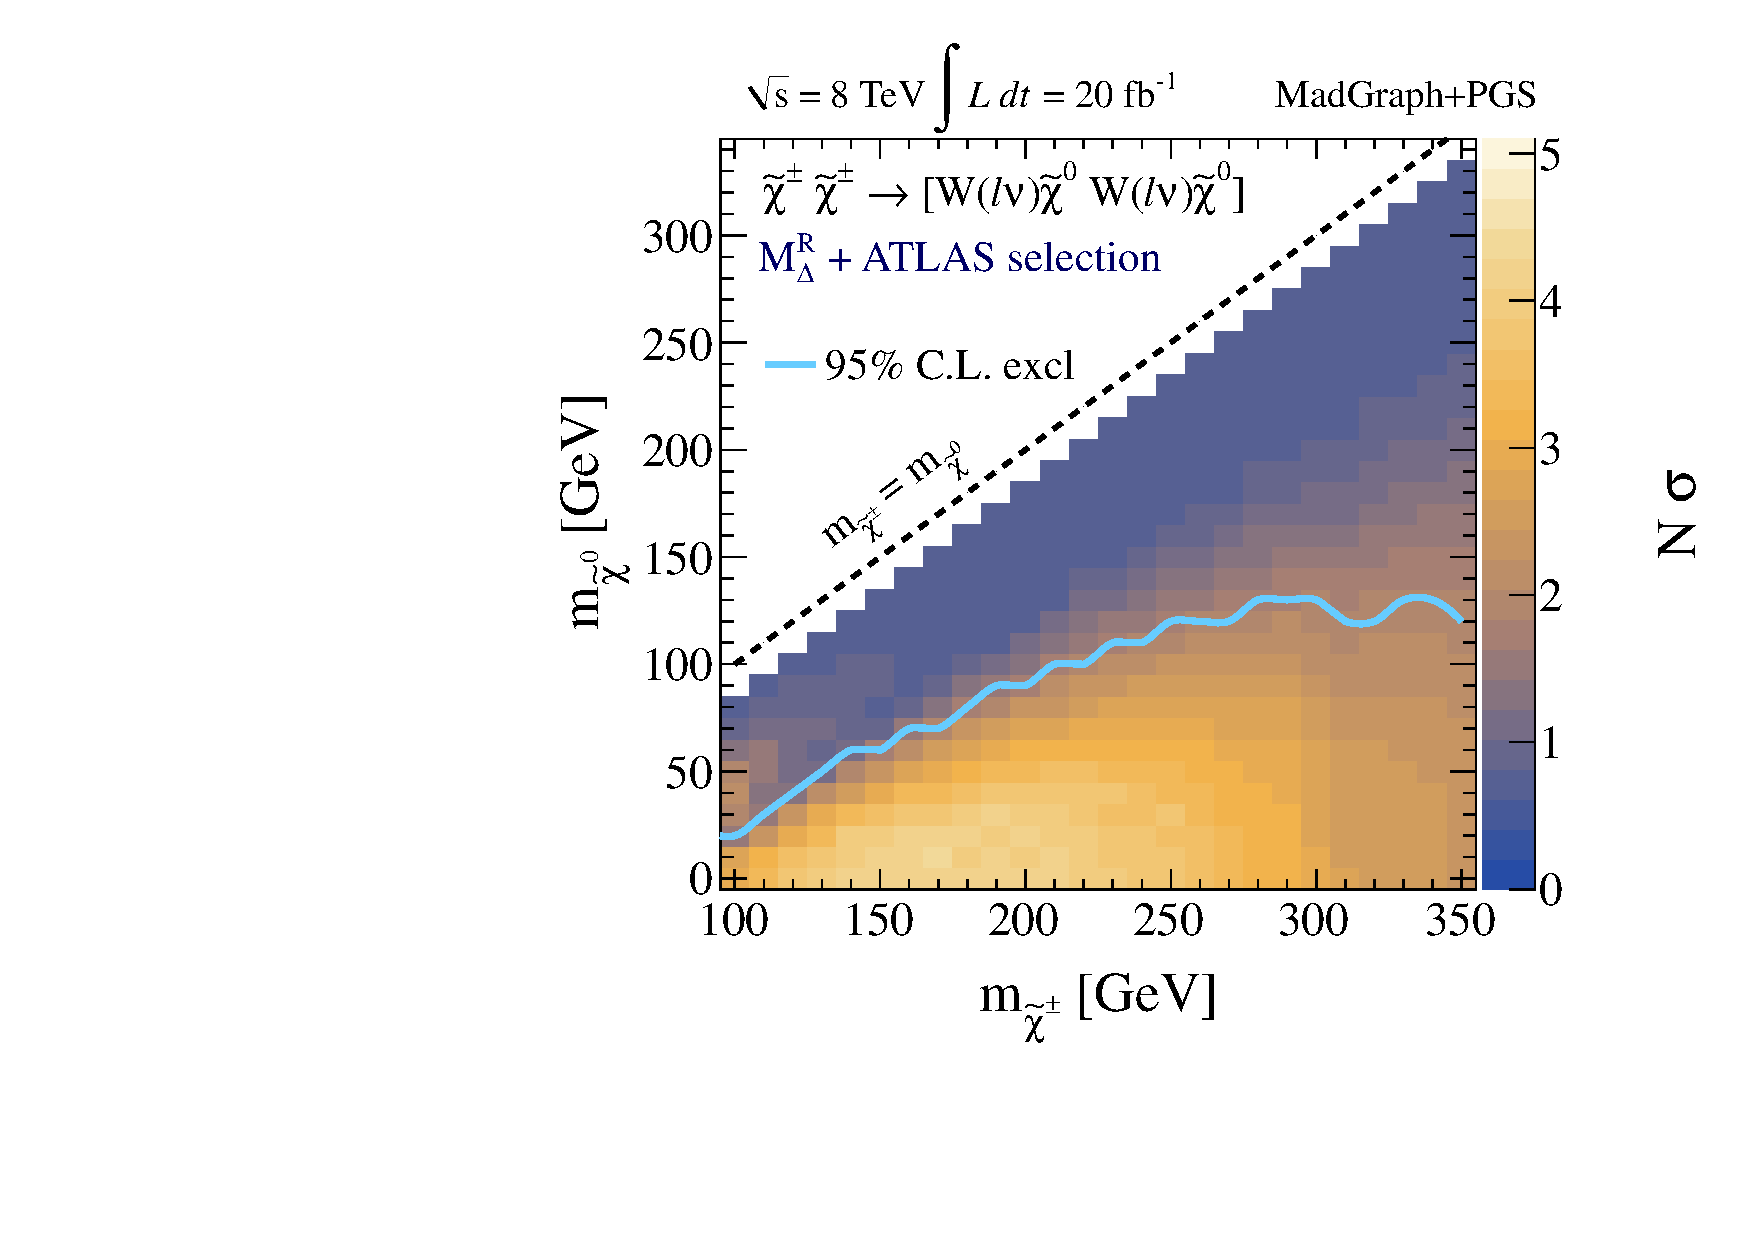
\includegraphics[width=0.4\columnwidth]{fig/sectionV/LIMIT2D_chargino_ATLAS_Mdelta.pdf}
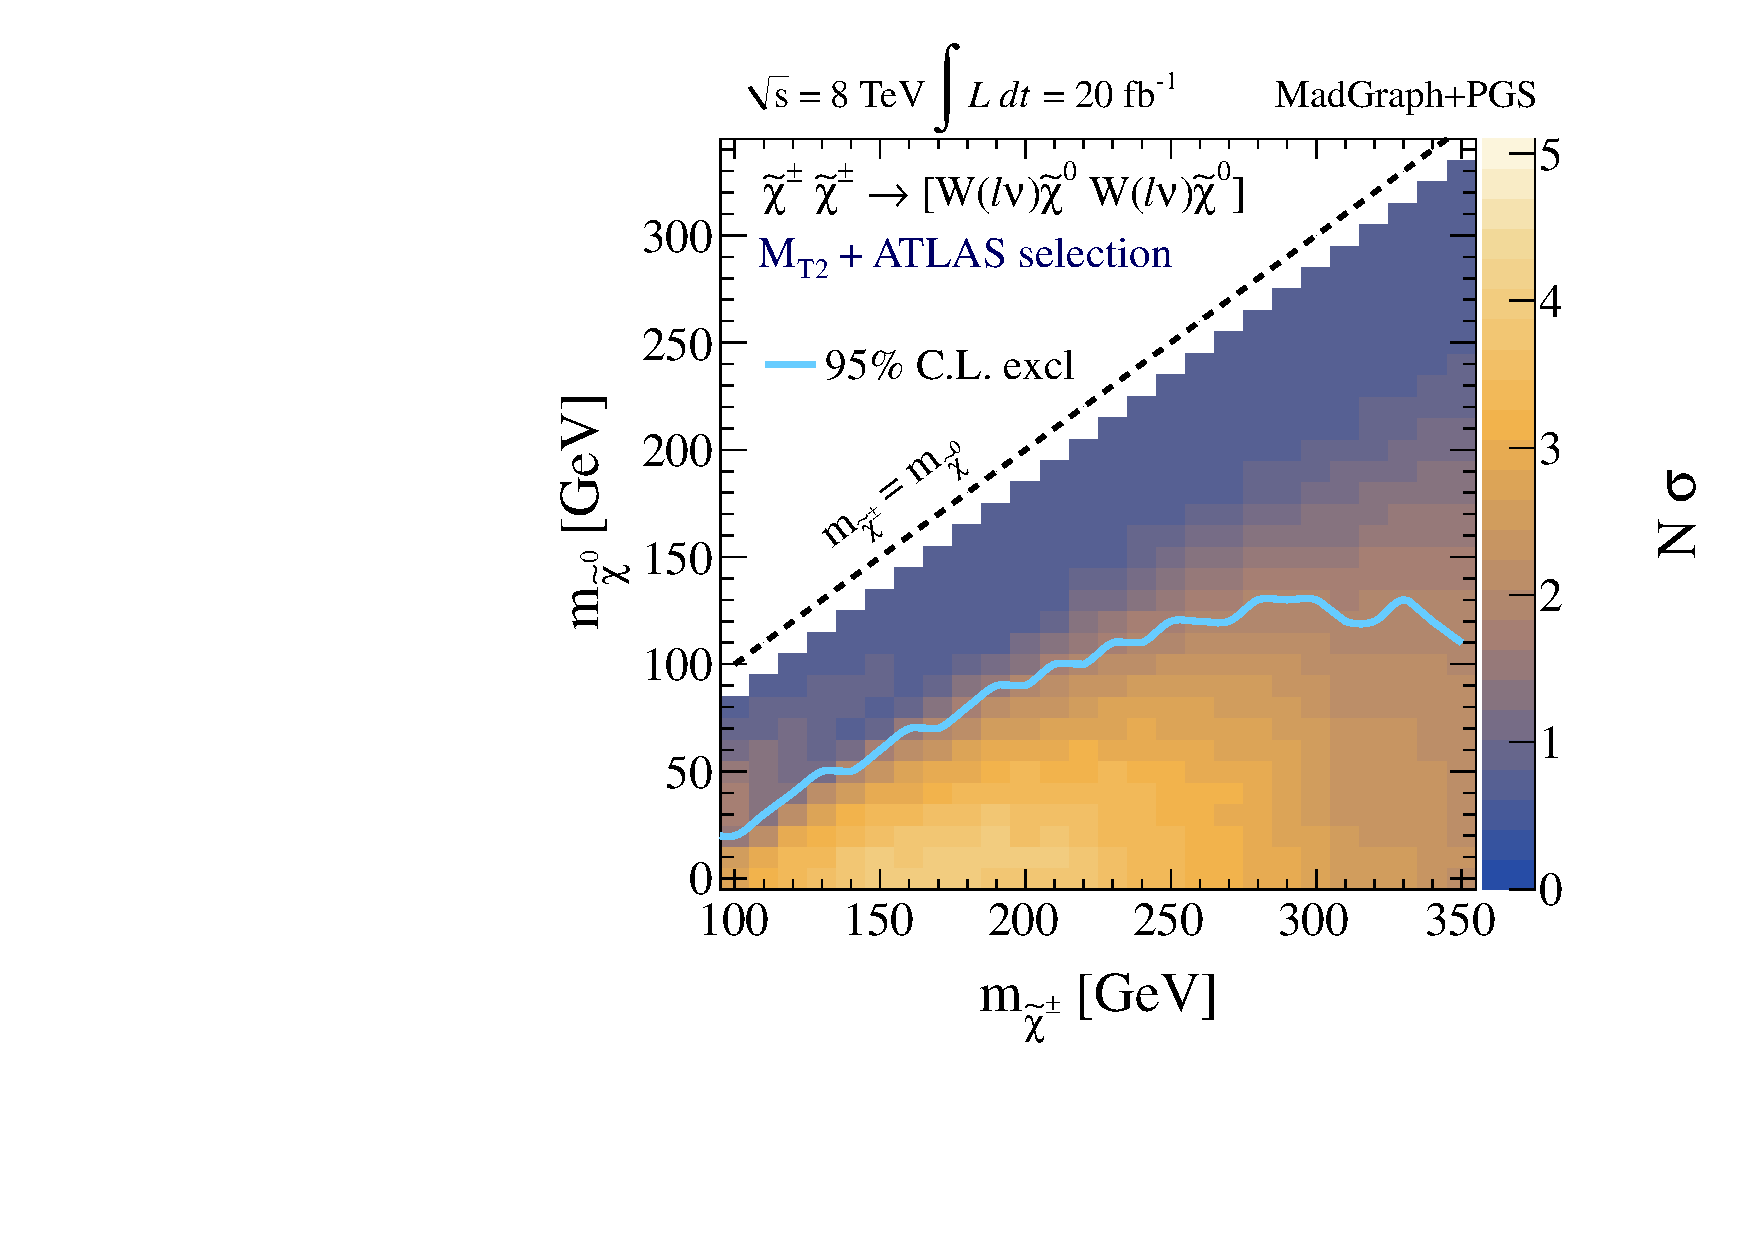
\includegraphics[width=0.4\columnwidth]{fig/sectionV/LIMIT2D_chargino_ATLAS_MT2.pdf}
\caption{Expected exclusion limits (in units of $\sigma$) for charginos decaying to neutralinos and leptonic $W$ bosons using 20~fb$^{-1}$ of 8 TeV data, as a function of both selectron and neutralino masses. Expected limits are shown for our 1D $M_\Delta^R$ analysis using CMS (upper left) and ATLAS (lower left) selection cuts, and directly compared to our expected exclusions using our simulated CMS $M_{CT\perp}$ (upper right) and ATLAS $M_{T2}$ (lower right) analyses.  \label{fig:results_chargino_2D_compare}}
\end{figure}

\begin{figure}[ht]
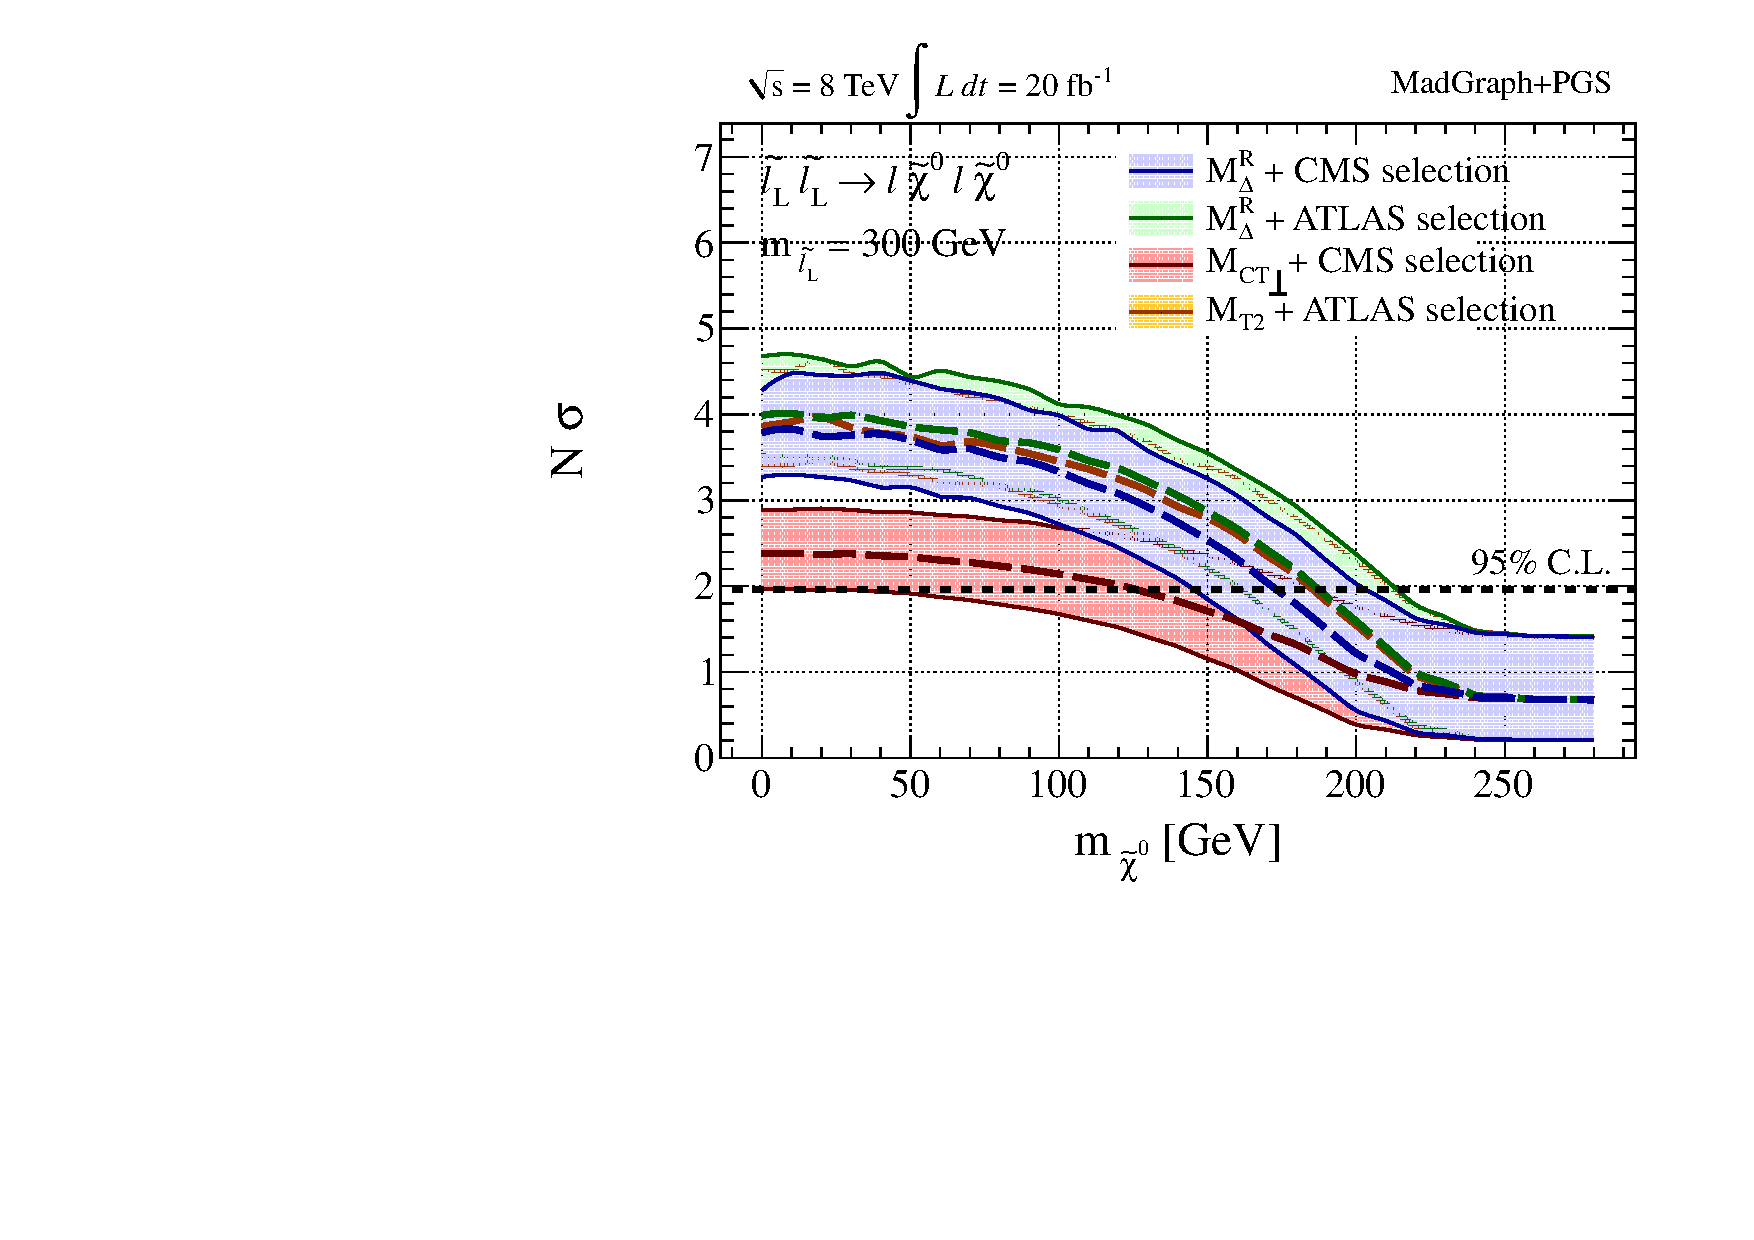
\includegraphics[width=0.4\columnwidth]{fig/sectionV/LIMIT1D_sleptonL_all_ML300.pdf}
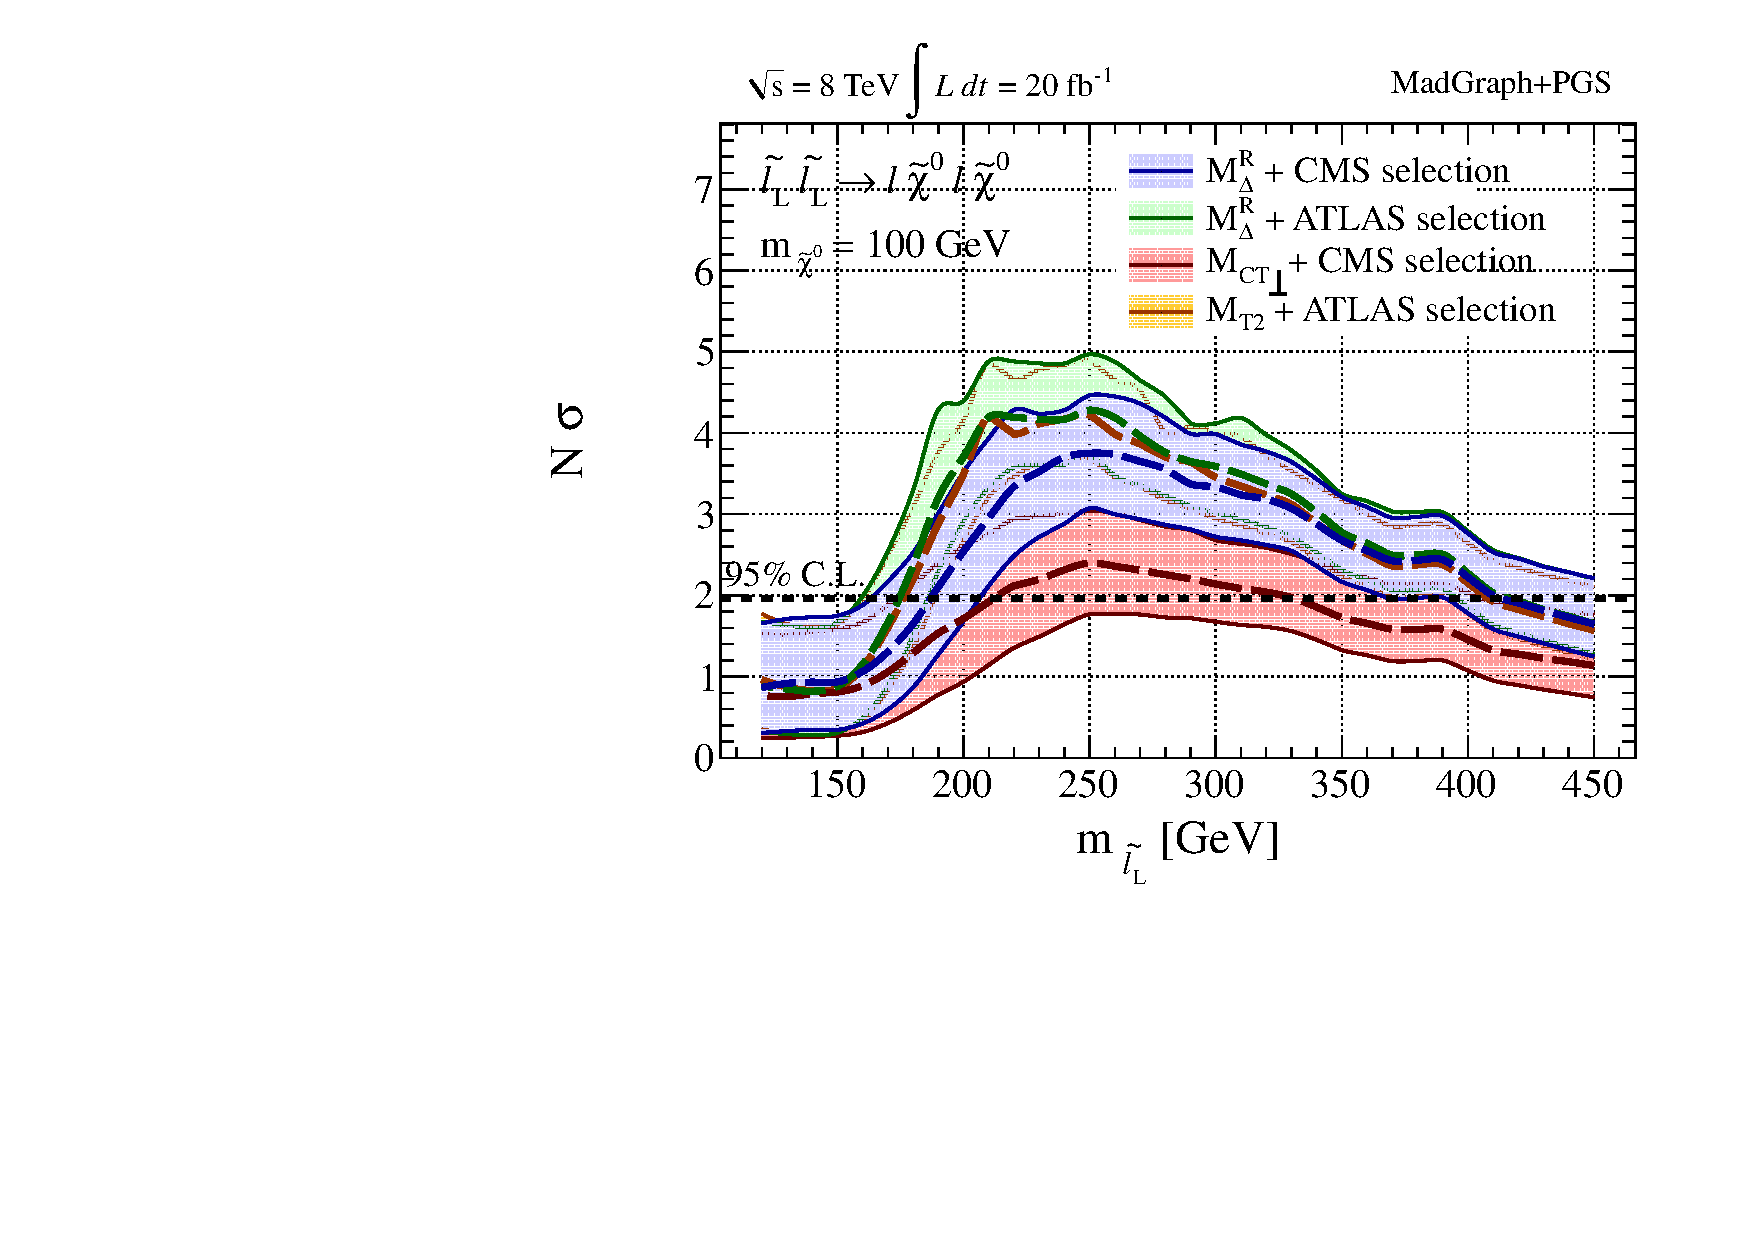
\includegraphics[width=0.4\columnwidth]{fig/sectionV/LIMIT1D_sleptonL_all_MX100.pdf}
\caption{Expected exclusion limits (in units of $\sigma$) for left-handed selectrons decaying to leptons and neutralinos using 20~fb$^{-1}$ of 8 TeV data, as a function of neutralino mass with 300 GeV selectrons (left) or as a function of selectron mass with 100 GeV neutralinos (right). Expected limits are shown for our 1D $M_\Delta^R$ analysis using CMS (blue) and ATLAS (green) selection cuts, and directly compared to our expected exclusions using our simulated CMS $M_{CT\perp}$ (red) and ATLAS $M_{T2}$ (orange) analyses. \label{fig:results_1D_compare}}
\end{figure}

\begin{figure}[ht]
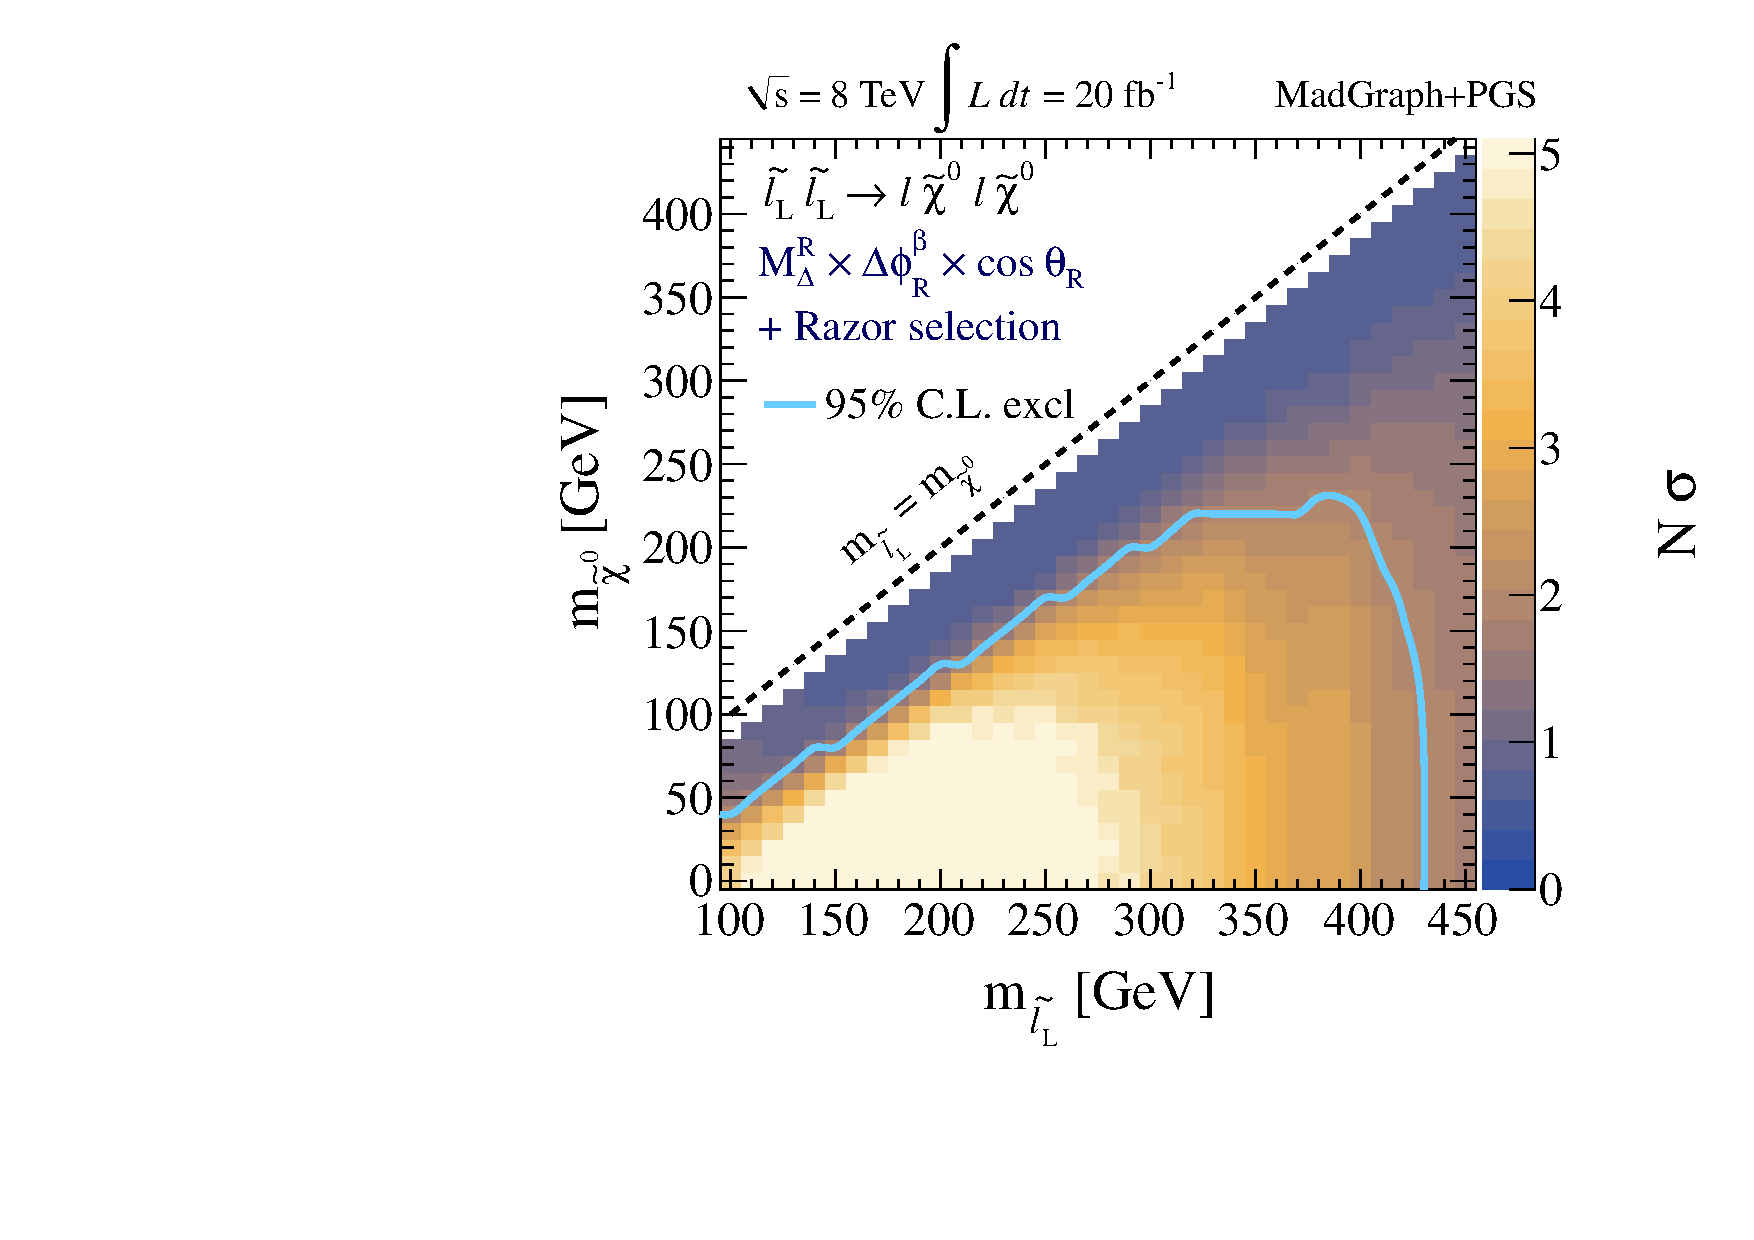
\includegraphics[width=0.4\columnwidth]{fig/sectionV/LIMIT2D_selectronL_Razor_MdeltaAngles.pdf}
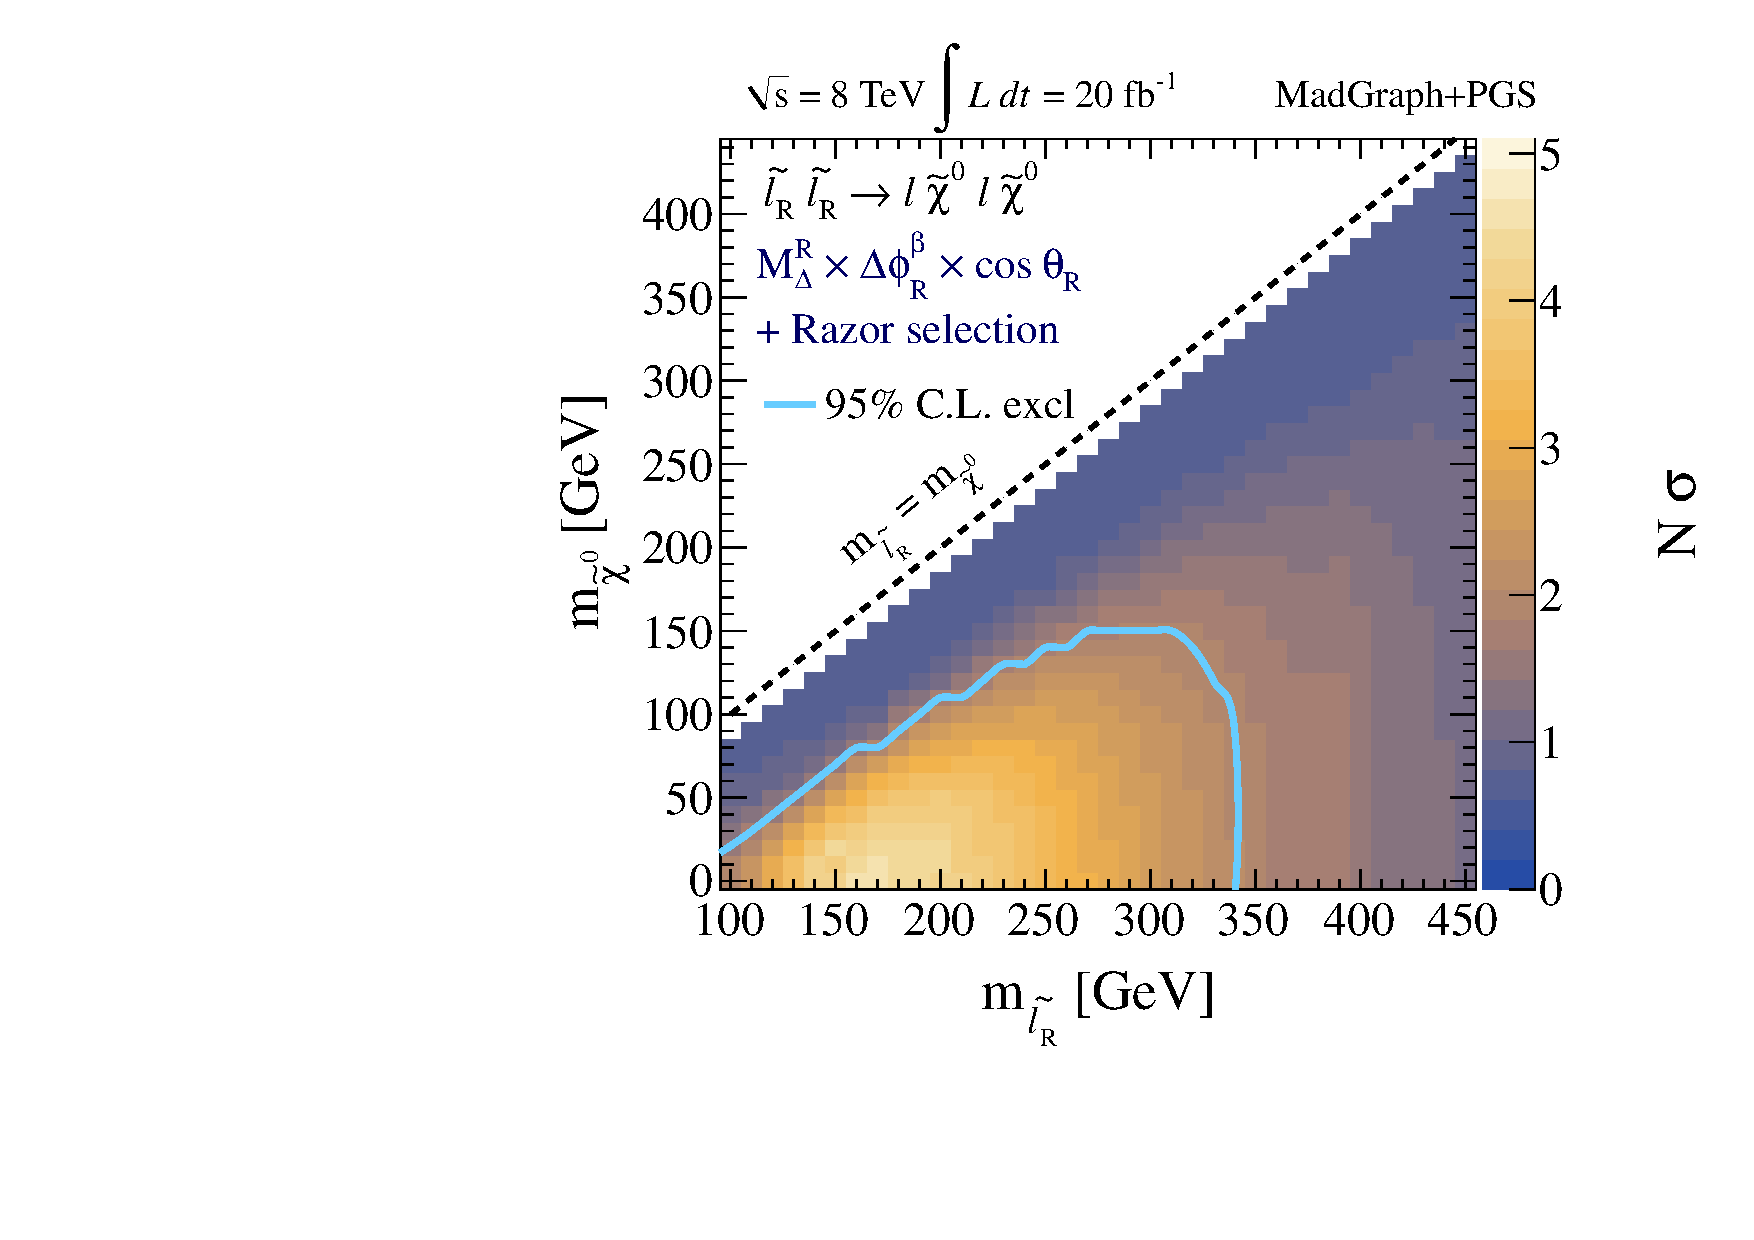
\includegraphics[width=0.4\columnwidth]{fig/sectionV/LIMIT2D_selectronR_Razor_MdeltaAngles.pdf}
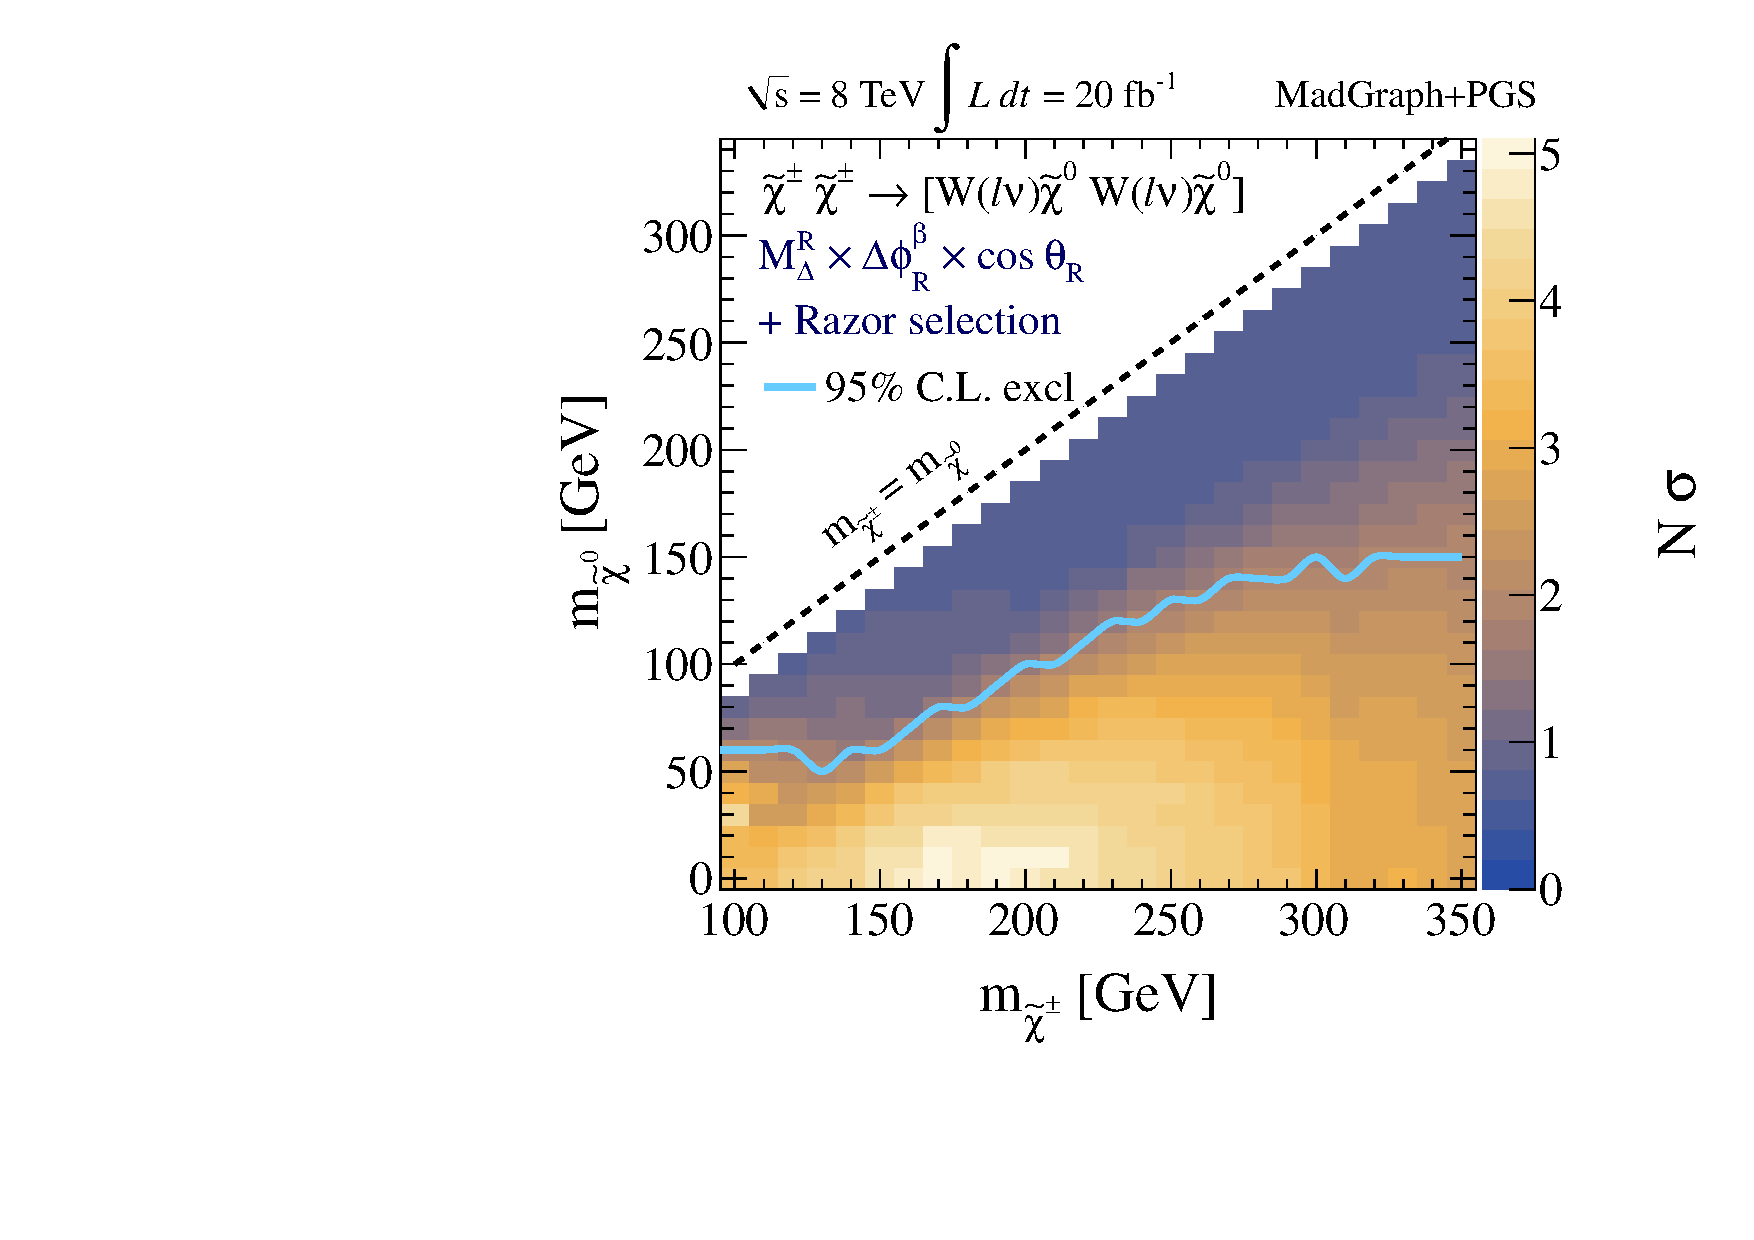
\includegraphics[width=0.4\columnwidth]{fig/sectionV/LIMIT2D_chargino_Razor_MdeltaAngles.pdf}
\caption{Expected exclusion limits (in units of $\sigma$) for left-handed selectrons (upper left) right-handed selectrons (upper right), and charginos decaying to neutralinos and leptonic $W$ bosons (bottom center) using 20~fb$^{-1}$ of 8 TeV data, as a function of both selectron/chargino and neutralino masses. Expected limits are derived using our multi-dimensional $M_\Delta^R$, $\Delta\phi_R^\beta$ and $|\cos\theta_{R+1}|$ analysis super-razor analyses with the razor selection cuts described in the previous section.  \label{fig:results_2D_best}}
\end{figure}


We can understand these 1D results by again consulting the kinematic distributions shown
in Figure \ref{fig:compare} of Section \ref{sec:simulation}. The fact that approximately 50\% of
signal events end up in the zero bin for $M_{CT\perp}$ gives a loss in statistics that is not
compensated by the clean kinematic edge. For $M_{T2}$ the corresponding effect is much smaller,
resulting in performance very similar to that achieved with $M_\Delta^R$.

In Figure~\ref{fig:results_2D_best}, we show the exclusion reach of the full super-razor analyses, using our multi-dimensional shape analysis which employs $M_\Delta^R$, $\Delta\phi_R^\beta$ and $|\cos\theta_{R+1}|$, and the new super-razor selection described in Section \ref{sec:shape} in order to maximize the sensitivity over background. Exclusions are shown for both left- and right-handed selectrons, as well as charginos decaying to $W$ bosons and neutralinos.  The exclusion sensitivities include the
effects from systematic errors on kinematic shapes, and on reconstruction of jets and leptons,
as described in Section \ref{sec:shape}. Again we emphasize that the
super-razor selection has no $E_{T}^\text{miss}$ cut.

Moderate improvements over the $M_\Delta^R$ analysis are visible for the selectrons, while the chargino sensitivity is greatly increased in the low-mass degeneracy regime. The relative improvements can be more clearly seen in the Figures~\ref{fig:results_slepton_1D_compare} and \ref{fig:results_chargino_1D_compare}, where we show the exclusion reach for fixed values of selectron/chargino or neutralino masses.

The super-razor improvements in the sensitivity to compressed spectra can be understood from
the additional kinematic information provided by the angles $\Delta\phi_R^\beta$ and $|\cos\theta_{R+1}|$. Recall that the magnitude of the approximate razor boost $\vec{\beta}_R$ is systematically larger than the correct boost $\vec{\beta}^{\, \rm CM}$, because of the the assumption that the energy of the event is evenly split between the visible and invisible systems. This causes a peaking of $\Delta\phi_R^\beta$ at $\pi$, since the sum of the visible momenta tends to be anti-aligned with the boost direction. As the spectrum becomes more and more compressed, this effect is magnified, as seen in Figure \ref{fig:dphi_v_dphi} of Section \ref{sec:variables}. Thus for compressed spectra  $\Delta\phi_R^\beta$ is a particularly good disciminator to appeal to in future searches.

As described in Section \ref{sec:variables}, $|\cos\theta_{R+1}|$ is related to the energy
difference of the leptons in the razor frame $R$, the approximation to the CM frame.
This difference is expected to be small for the Drell-Yans + jets background, and is also
peaked at zero for the $W^-W^+$ background, because of polarization effects.
For signal events the distributions in $|\cos\theta_{R+1}|$ are much flatter; the
polarization effects are absent either because the parent particles are spin zero
(sleptons) or because we have two-step decays (charginos).

Each of the super-razor variables, $M_{\Delta}^{R}$, $\sqrt{\hat{s}}_{R}$, $\vec{\beta}_{R}$, $\vec{\beta}_{R+1}$, $\Delta \phi_{R}^{\beta}$, 
$|\cos\theta_{R+1}|$, and the angle $|\Delta\phi (\vec{p}_{\ell\ell}^{\, \text{lab}},\vec{E}_{T}^\text{miss})|$
used in the super-razor selection,
represents a different piece of information about an event.
The collection can be thought of as a kinematic basis, which raises the question of whether one
can identify an optimal kinematic basis for a particular type of search, e.g. searches for
sleptons with compressed spectra. The answer to this question depends not just on the
kinematic properties of the signal, but also on kinematics of the major backgrounds and
especially on the detector effects that dominate the systematic uncertainties. It seems plausible that in some cases there may be a family of approximately equivalent kinematic bases, such that
more or less the same kinematic information is exploited in different ways but resulting in
approximately equivalent sensitivity. 




\begin{figure}[!ht]
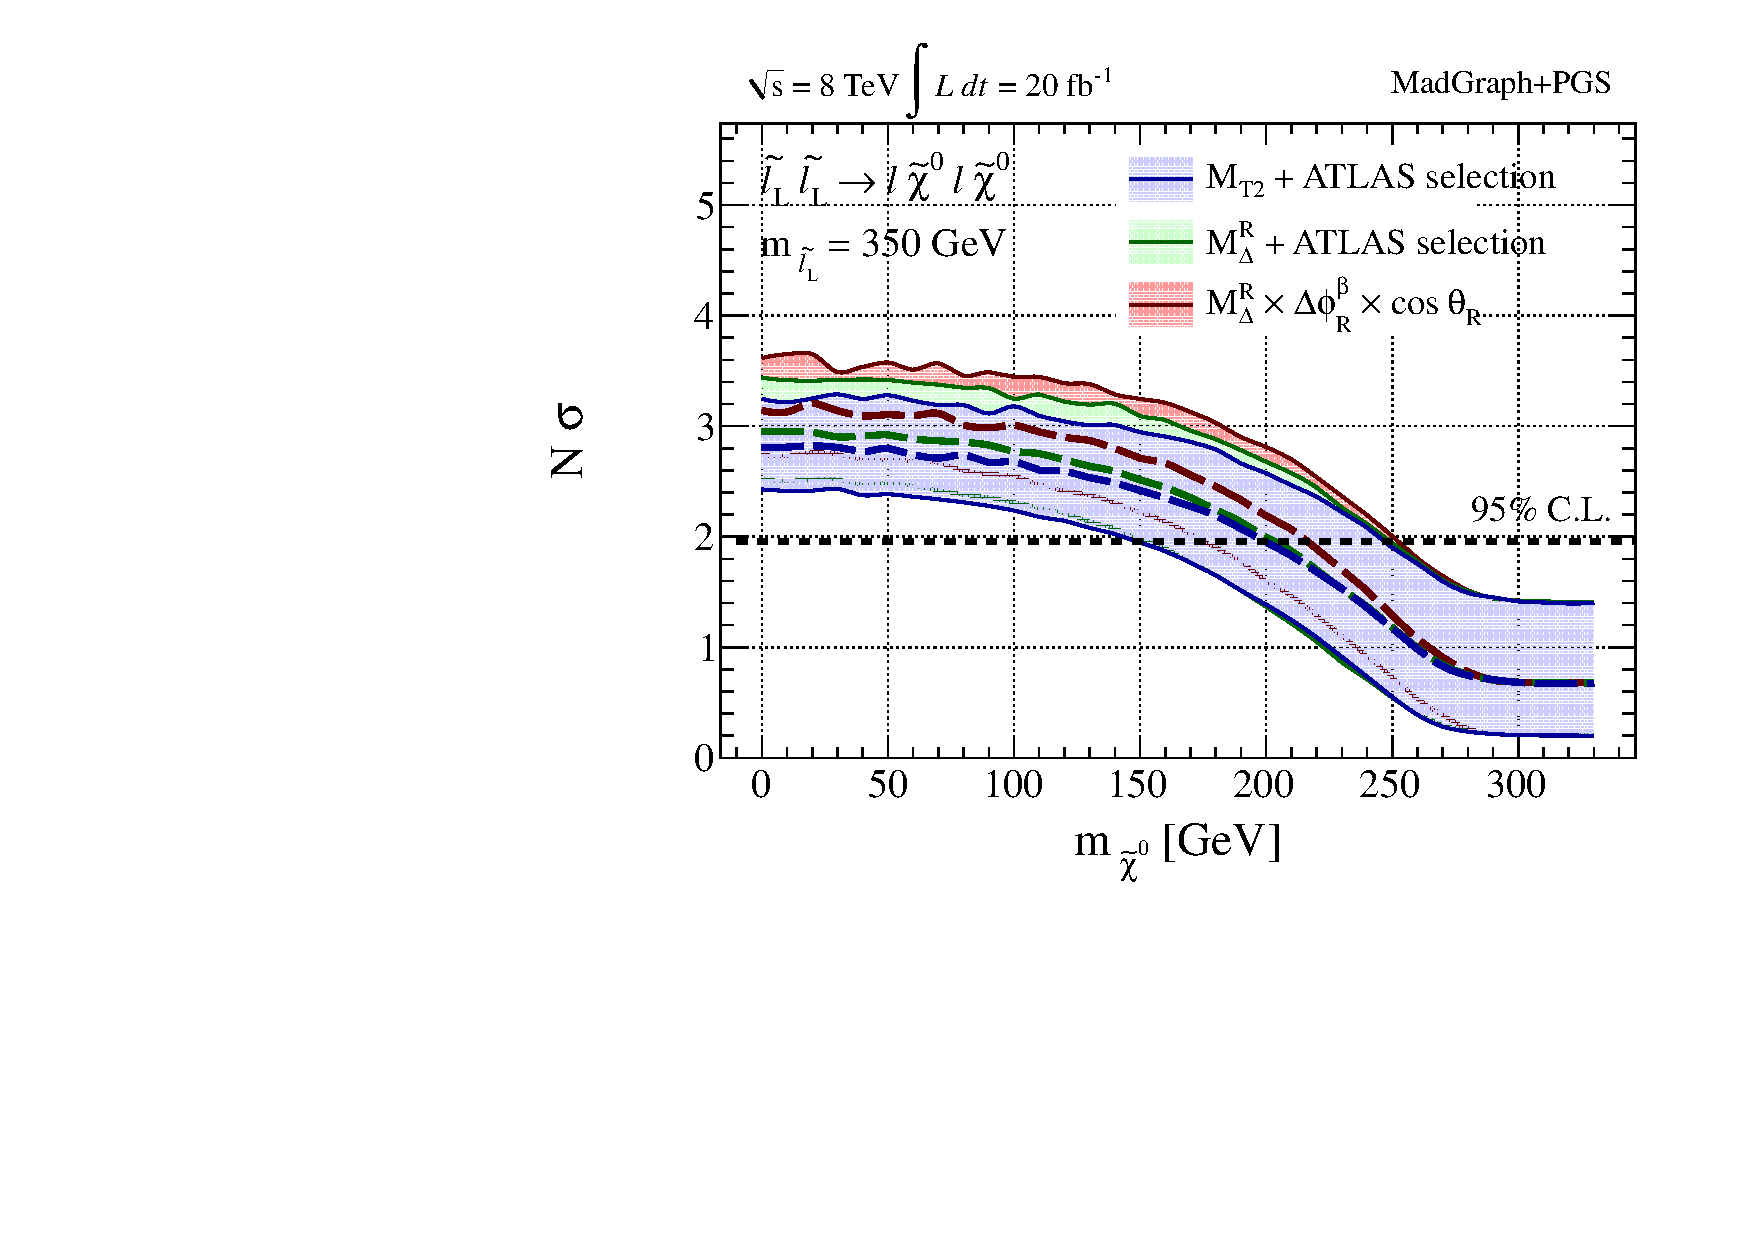
\includegraphics[width=0.40\columnwidth]{fig/sectionV/LIMIT1D_sleptonL_ATLAS_ML350.pdf}
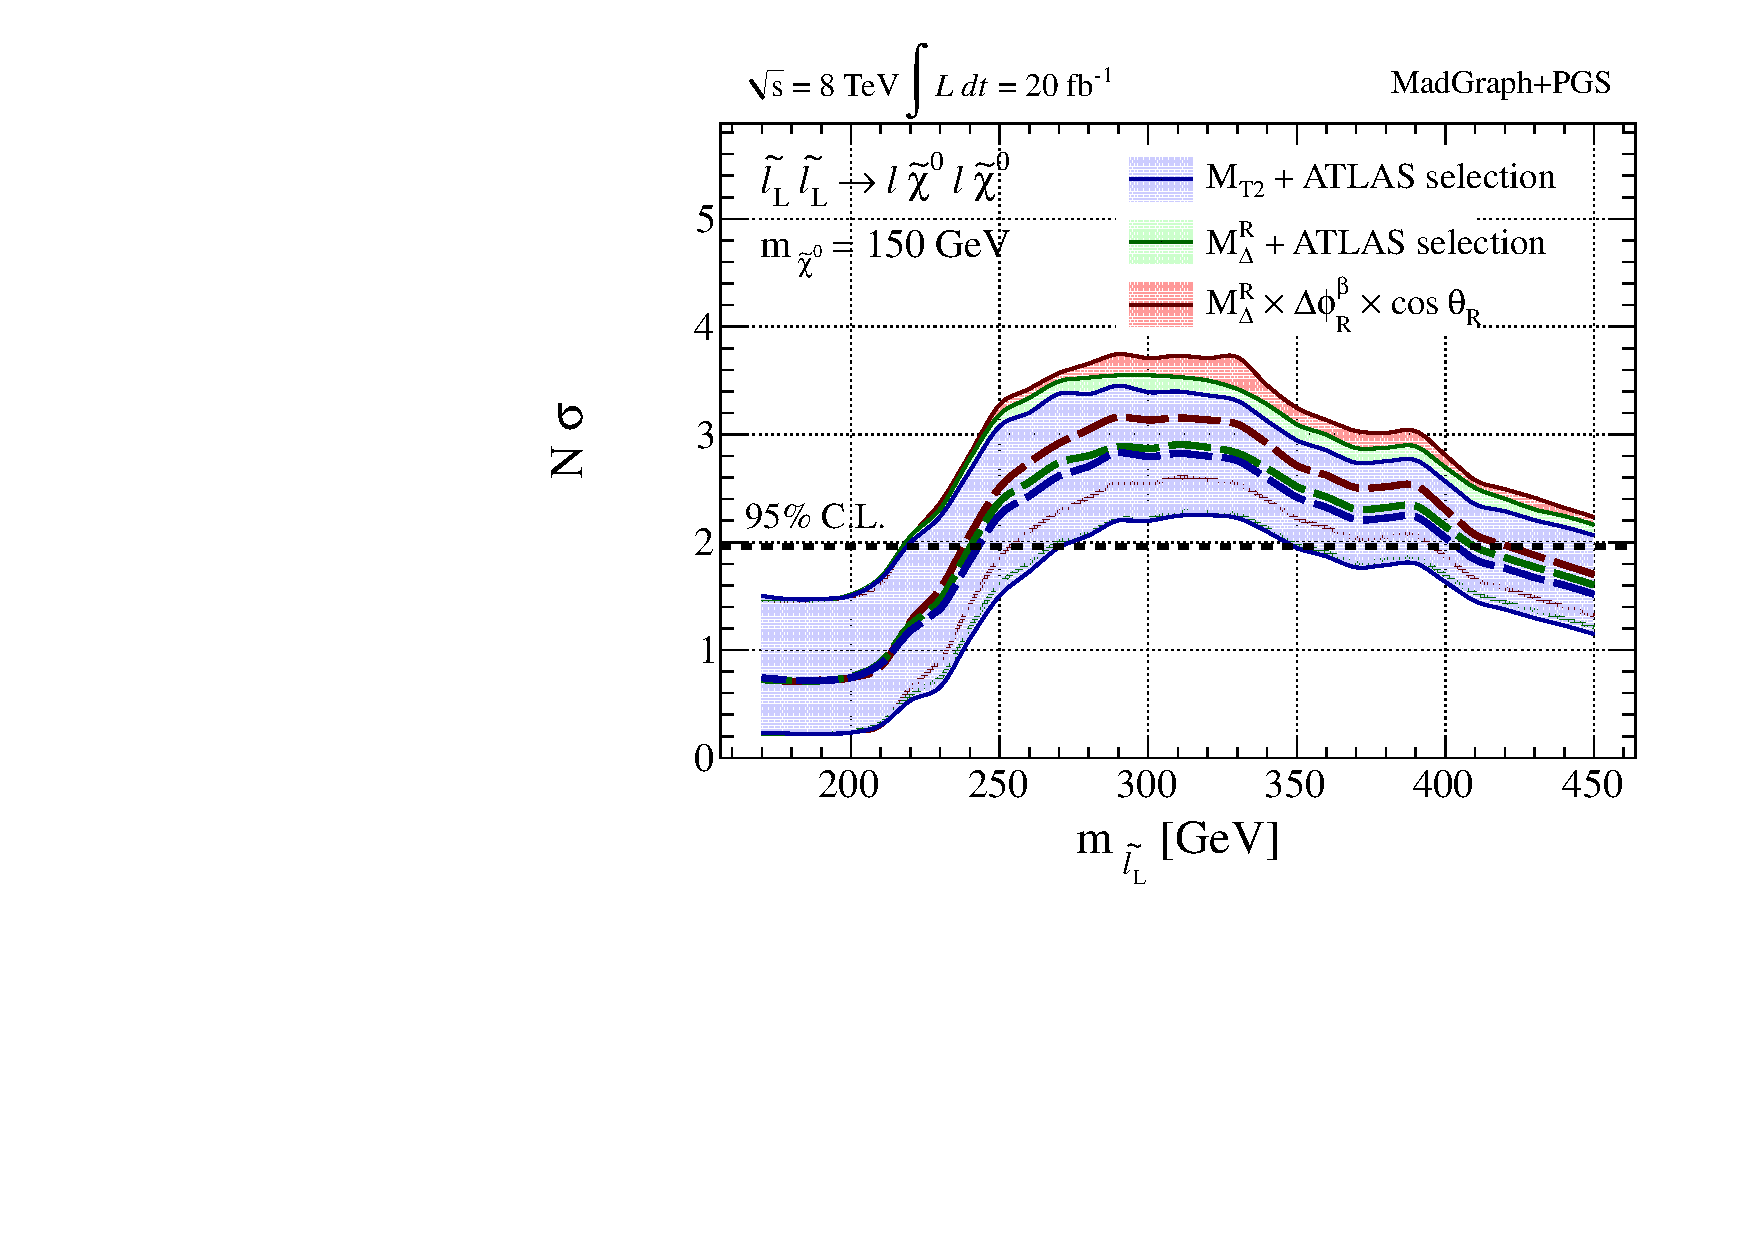
\includegraphics[width=0.40\columnwidth]{fig/sectionV/LIMIT1D_sleptonL_ATLAS_MX150.pdf}
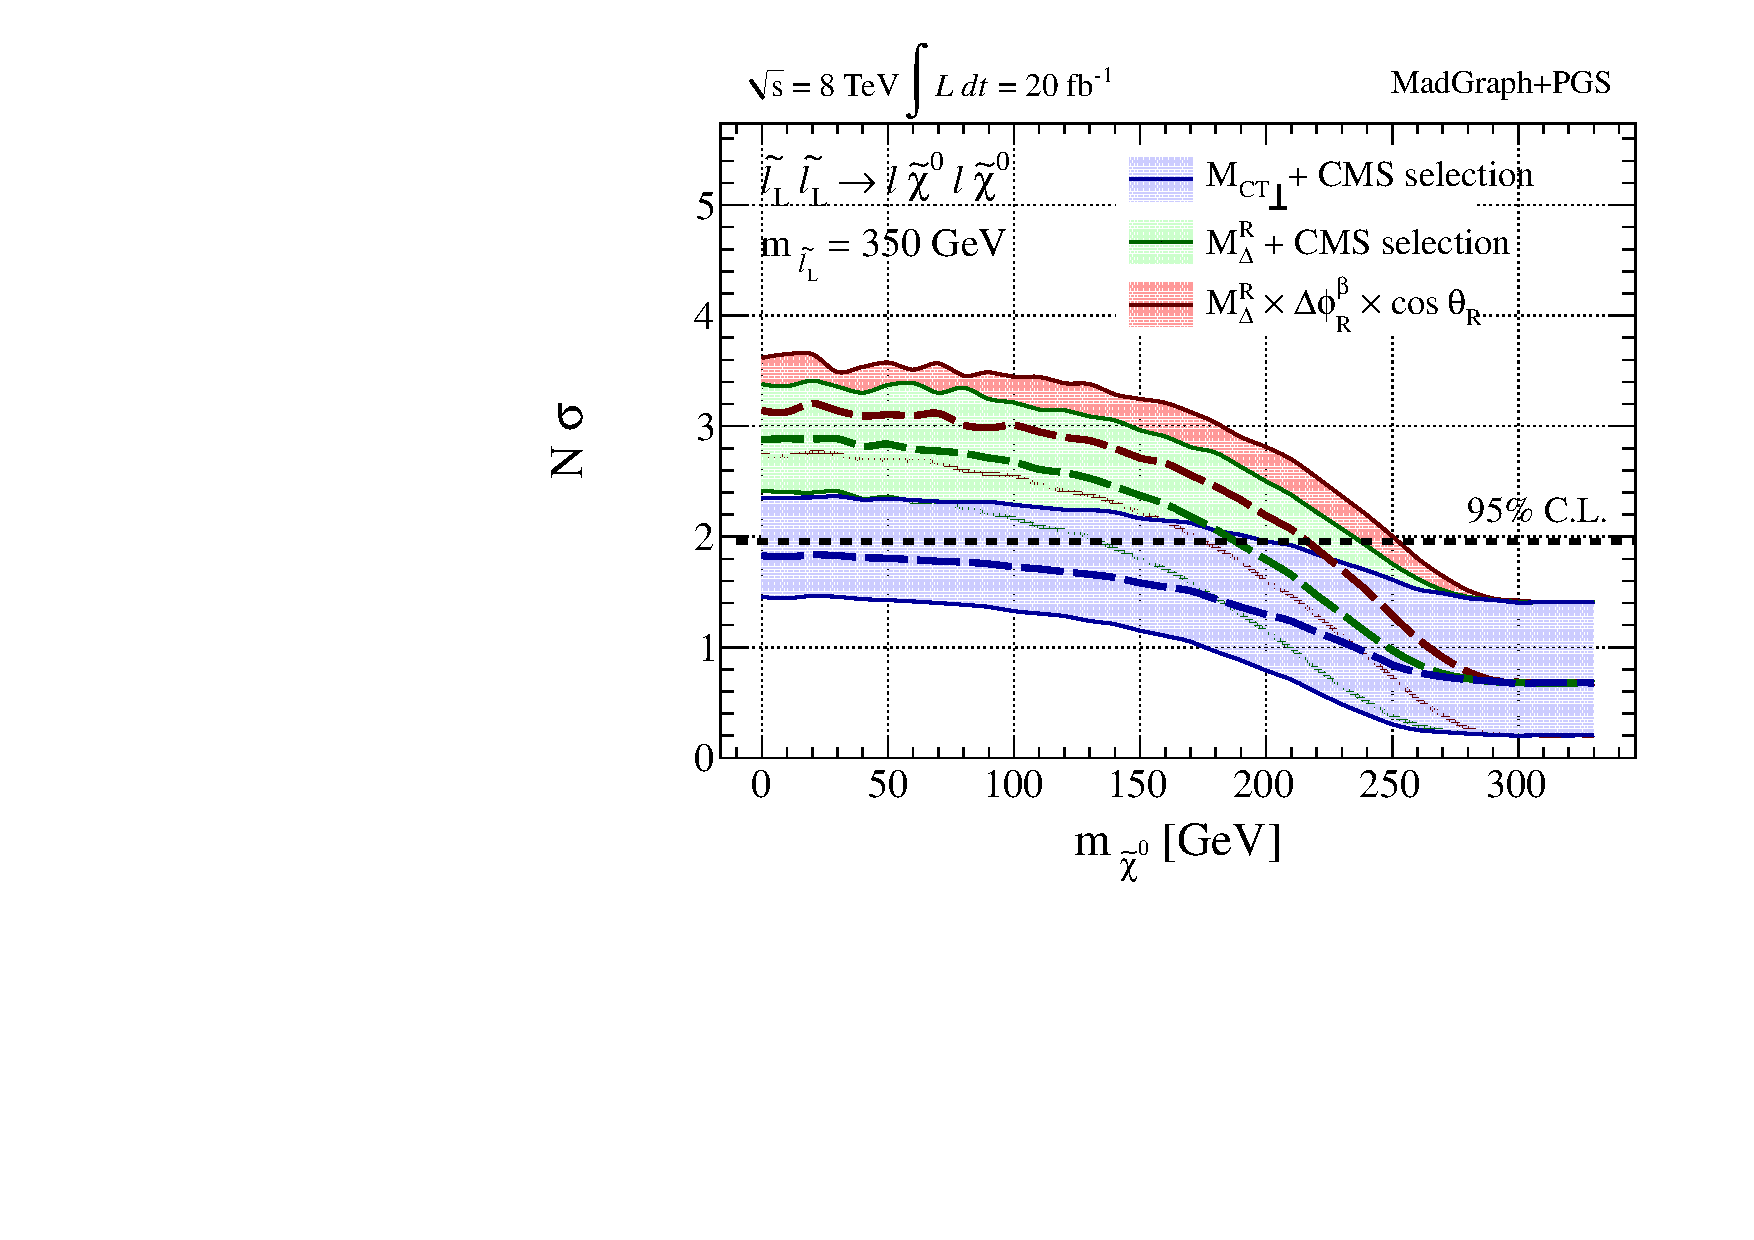
\includegraphics[width=0.40\columnwidth]{fig/sectionV/LIMIT1D_sleptonL_CMS_ML350.pdf}
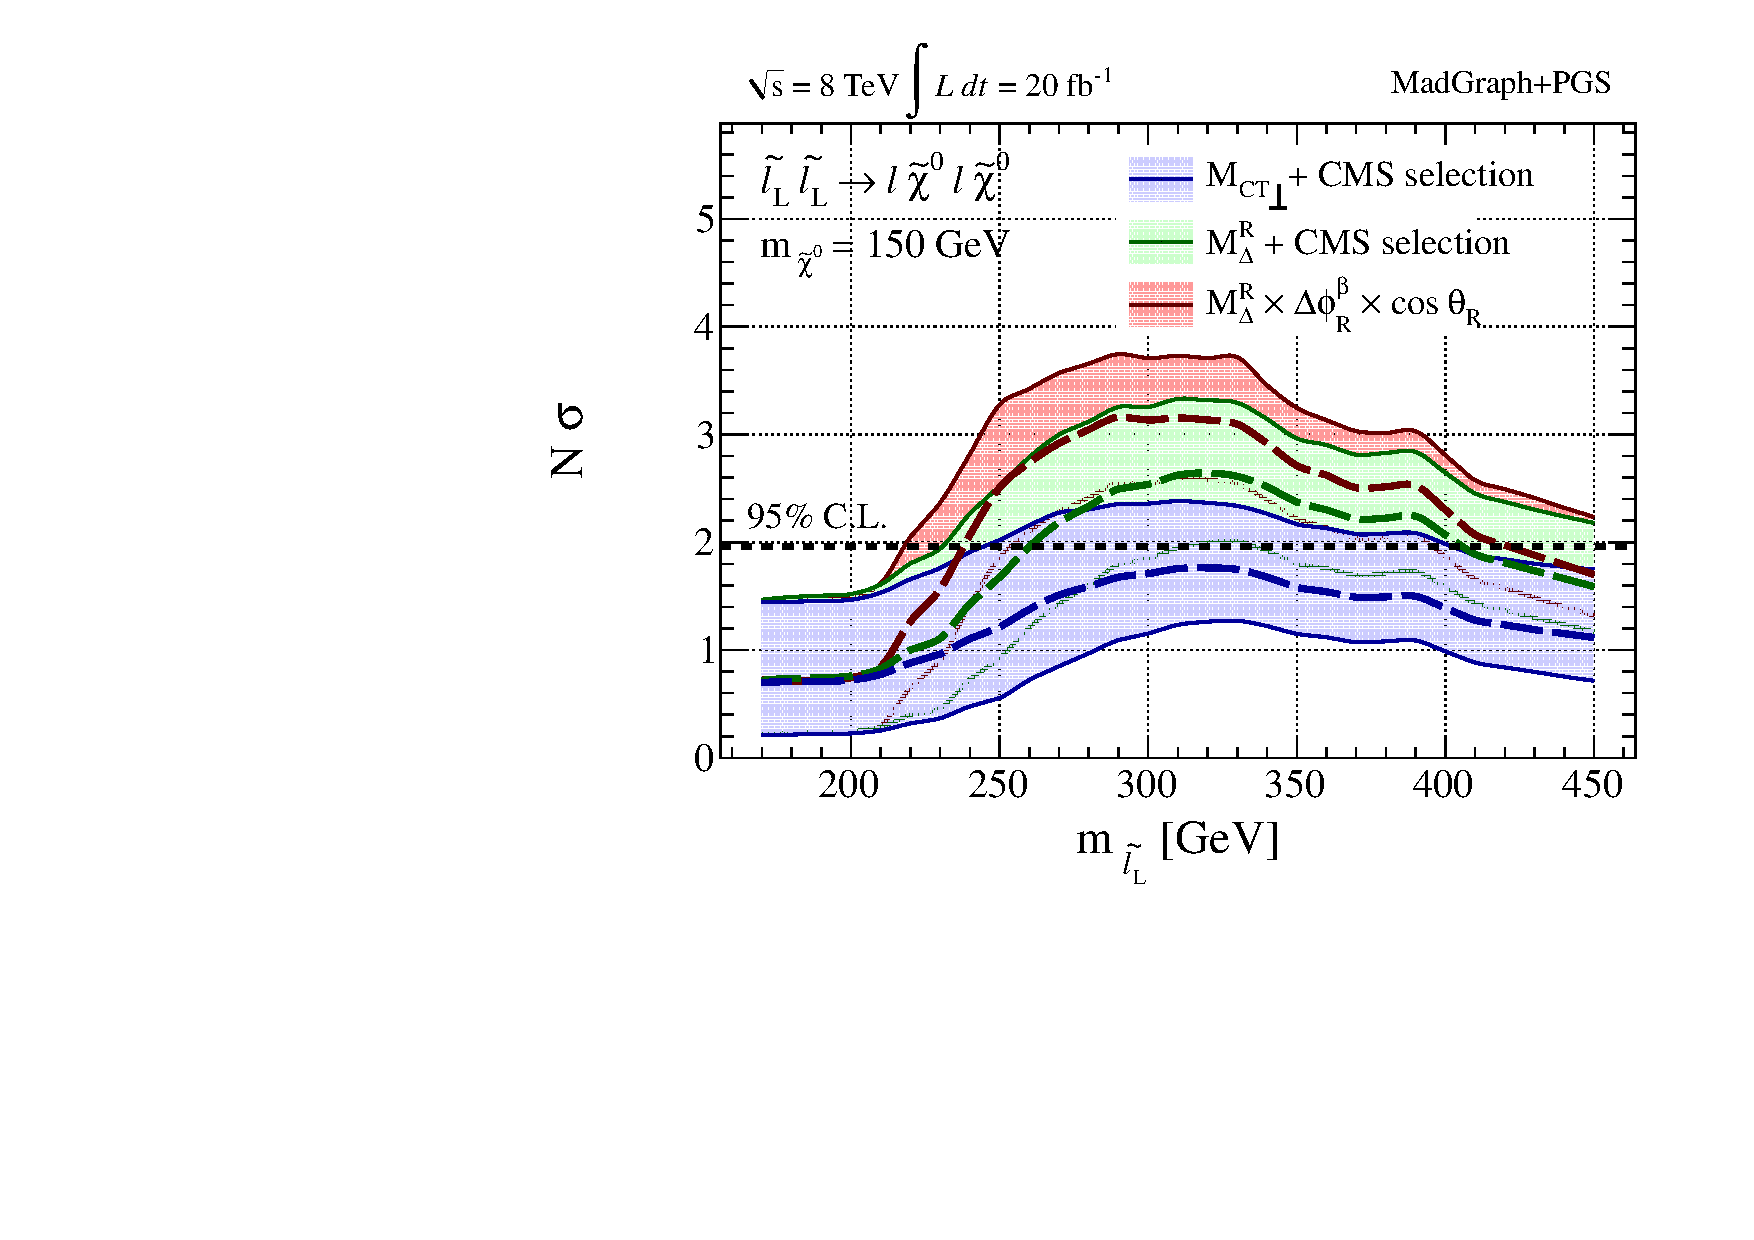
\includegraphics[width=0.40\columnwidth]{fig/sectionV/LIMIT1D_sleptonL_CMS_MX150.pdf}
\caption{Expected exclusion limits (in units of $\sigma$) for left-handed selectrons decaying to leptons and neutralinos using 20~fb$^{-1}$ of 8 TeV data, as a function of neutralino mass with 350 GeV selectrons (upper and lower left) or as a function of selectron mass with 150 GeV neutralinos (upper and lower right). Expected limits are shown for our multi-dimensional razor analysis (red), and compared to either ATLAS (upper plots) or CMS (lower plots) mass variables and selection criteria. \label{fig:results_slepton_1D_compare}}
\end{figure}

\begin{figure}[!hb]
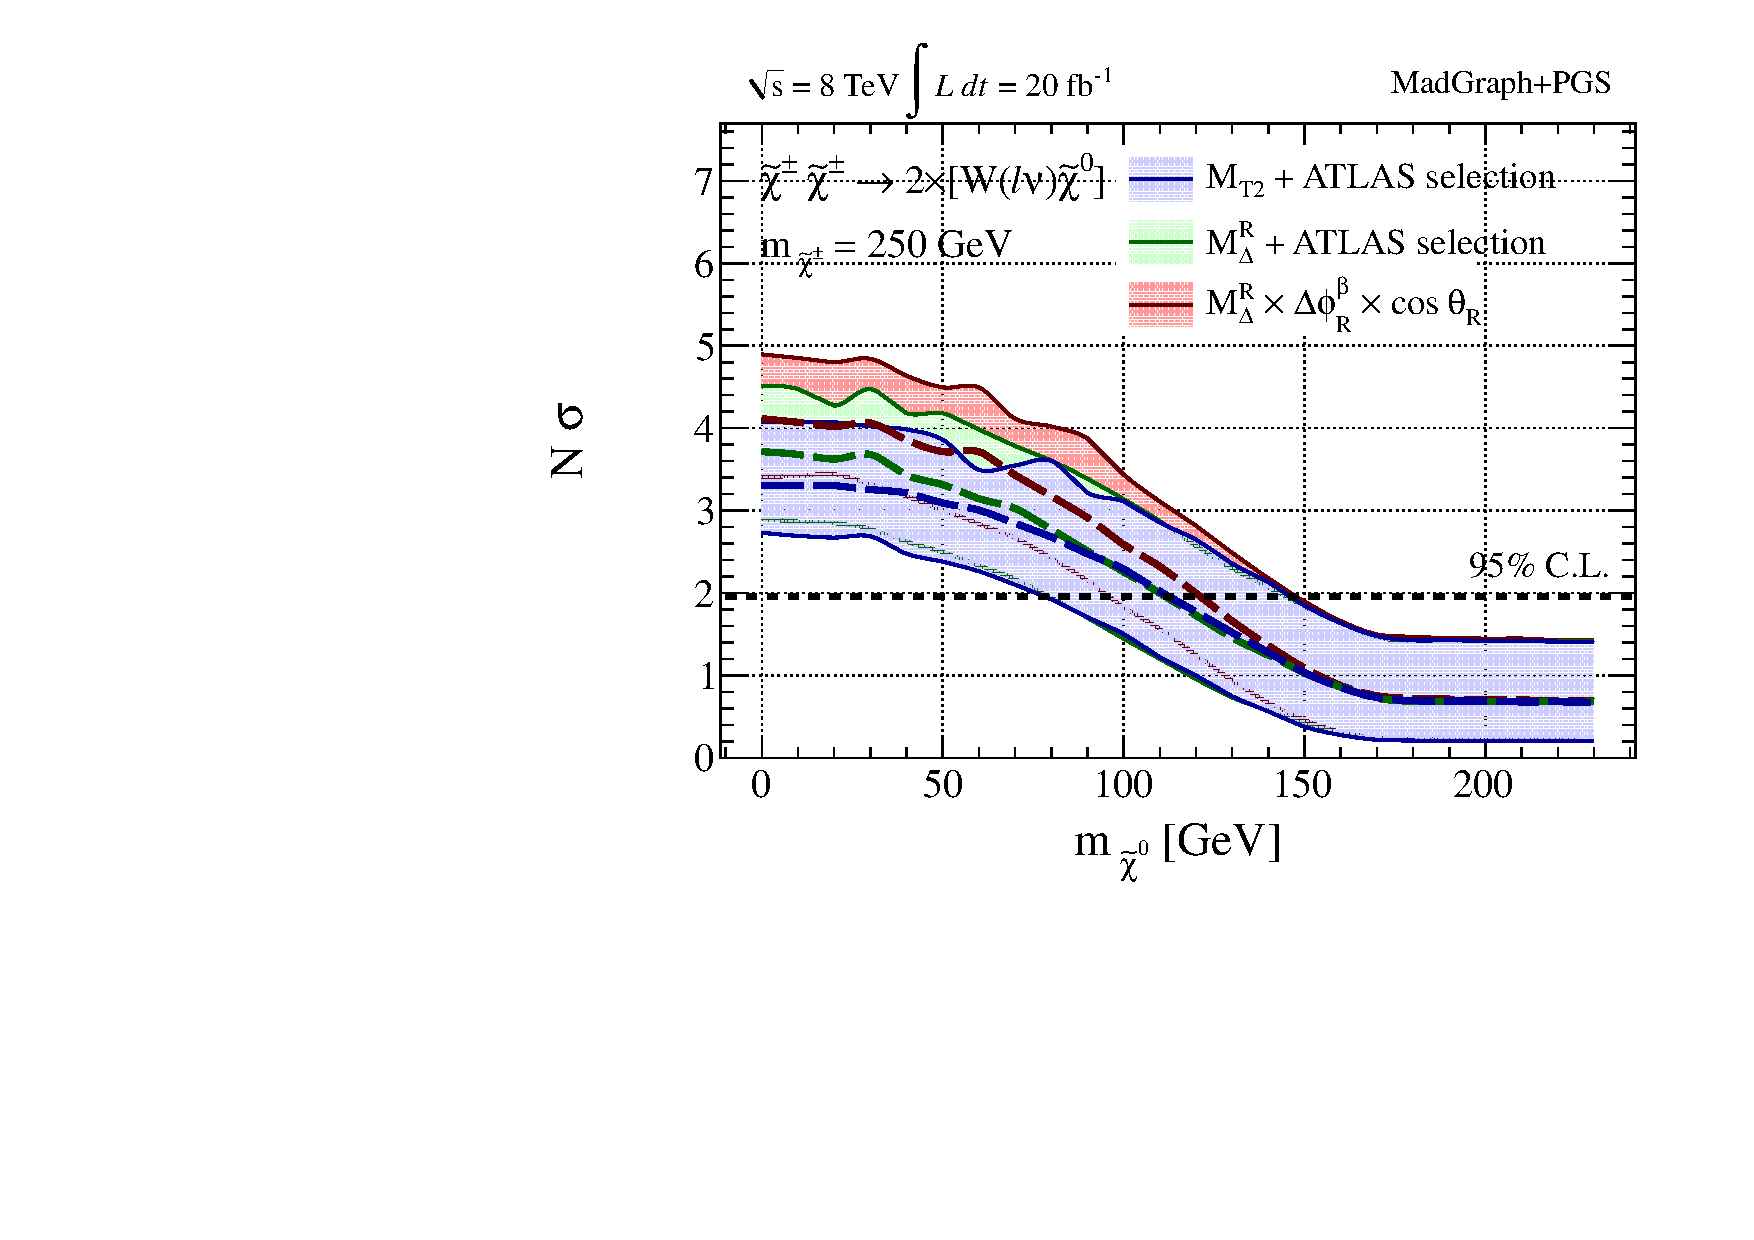
\includegraphics[width=0.40\columnwidth]{fig/sectionV/LIMIT1D_chargino_ATLAS_MXpm250.pdf}
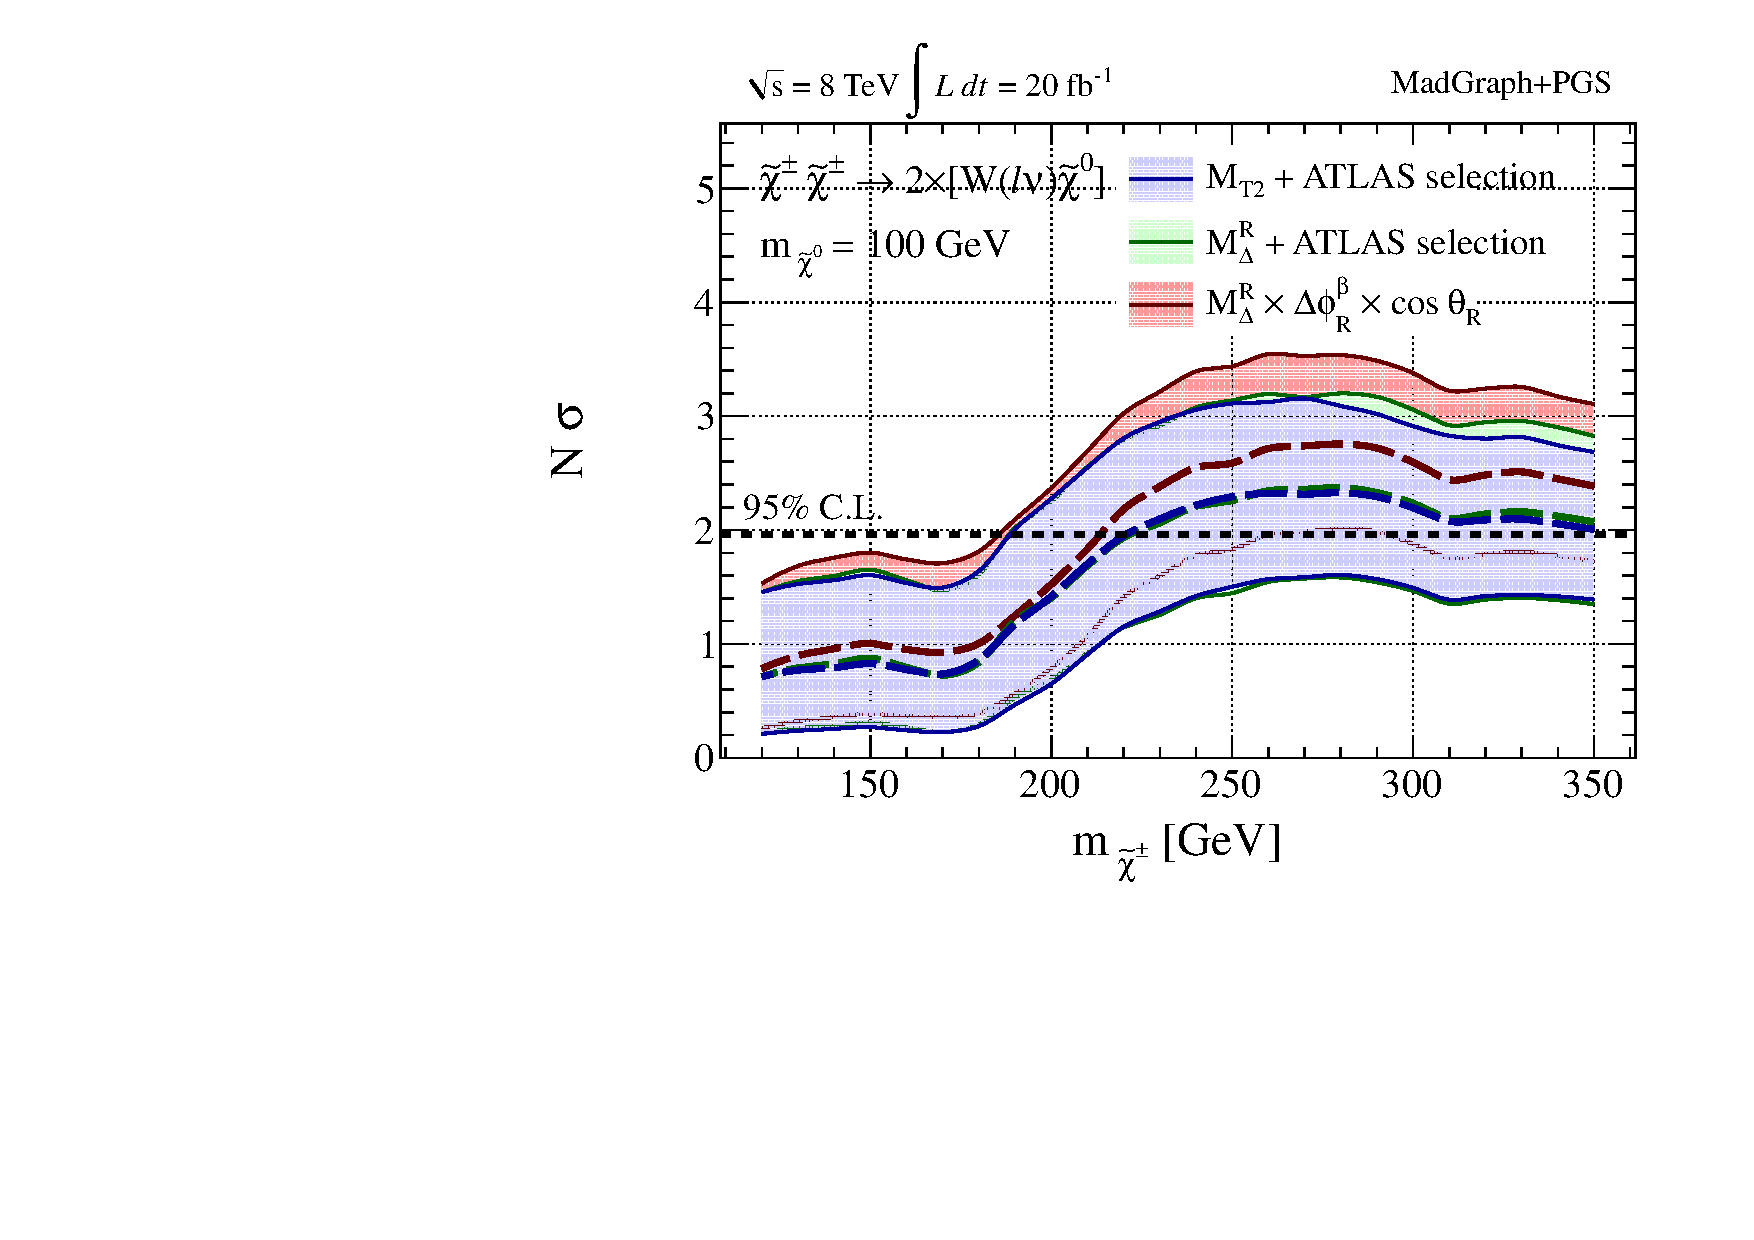
\includegraphics[width=0.40\columnwidth]{fig/sectionV/LIMIT1D_chargino_ATLAS_MX0100.pdf}
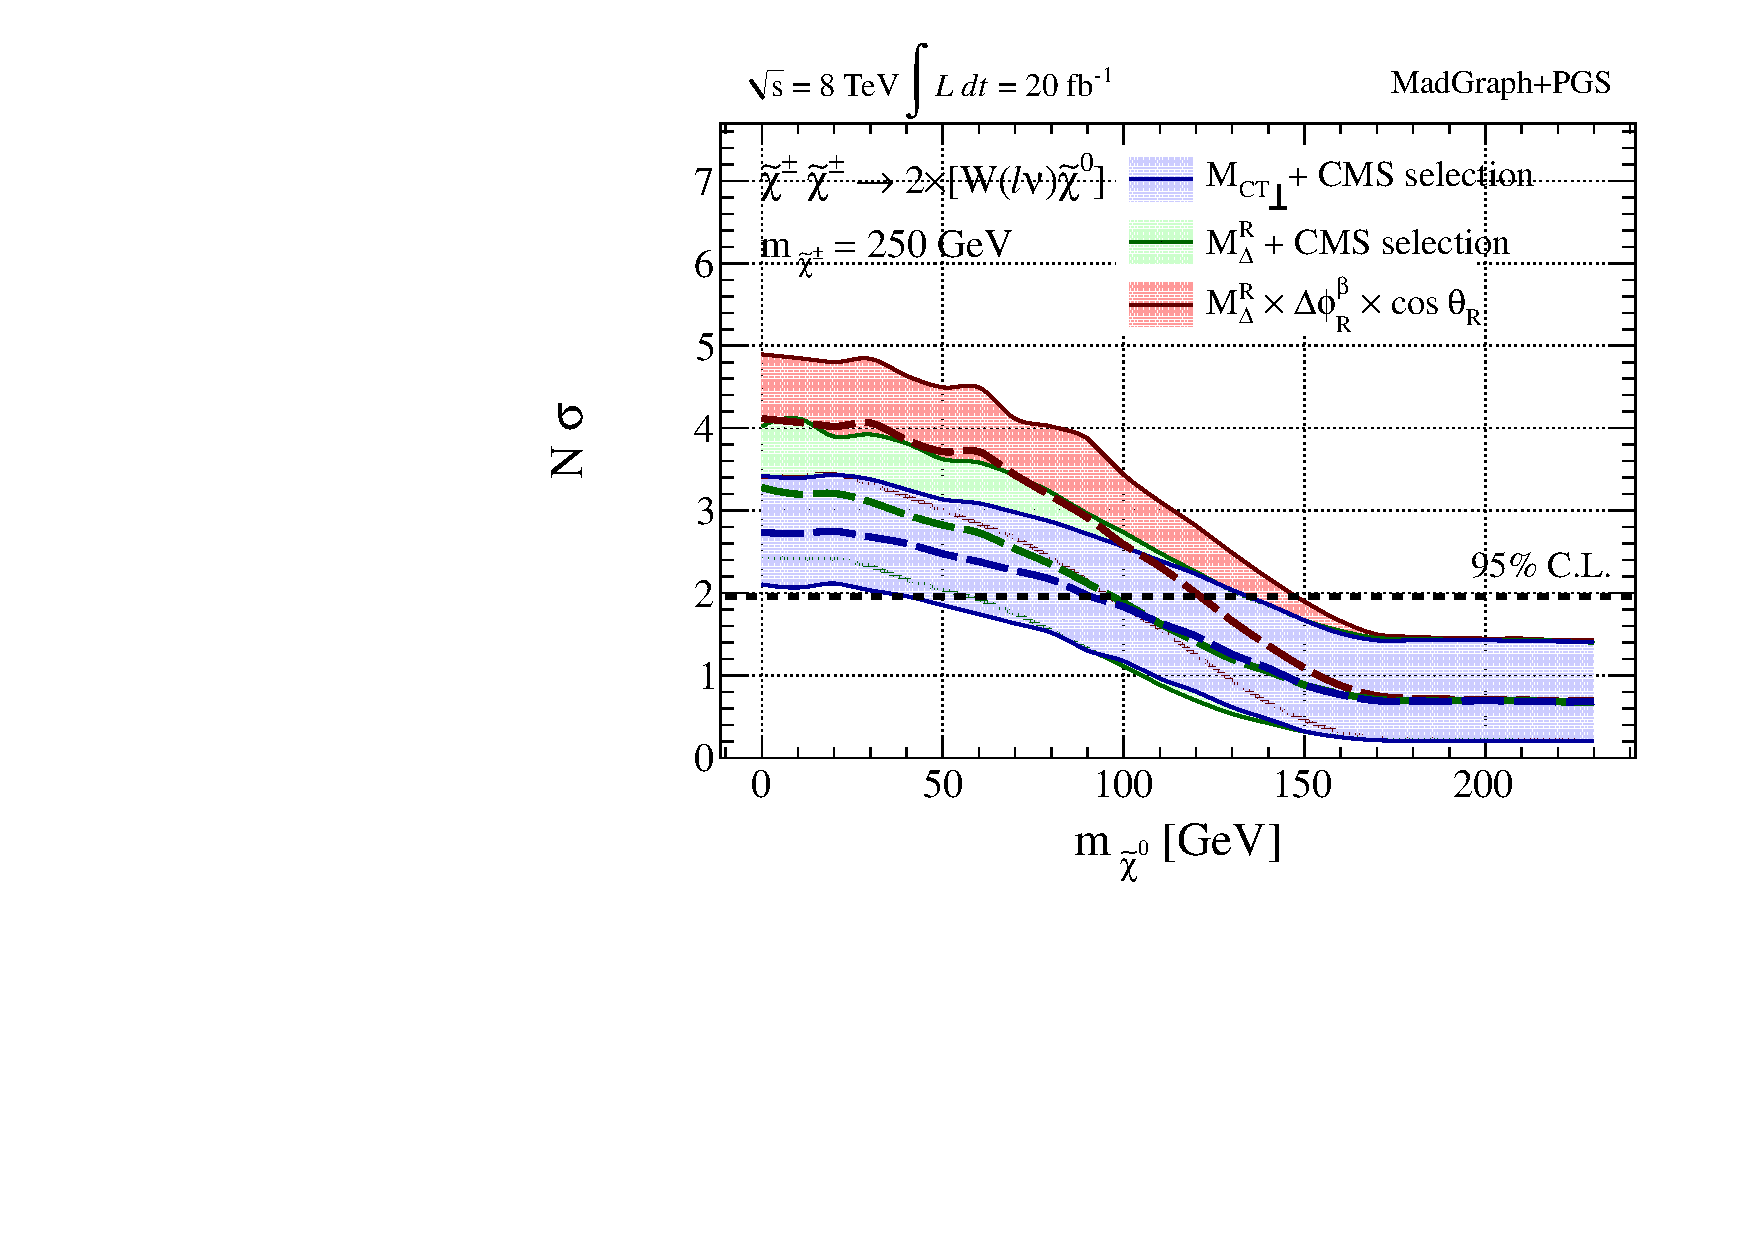
\includegraphics[width=0.40\columnwidth]{fig/sectionV/LIMIT1D_chargino_CMS_MXpm250.pdf}
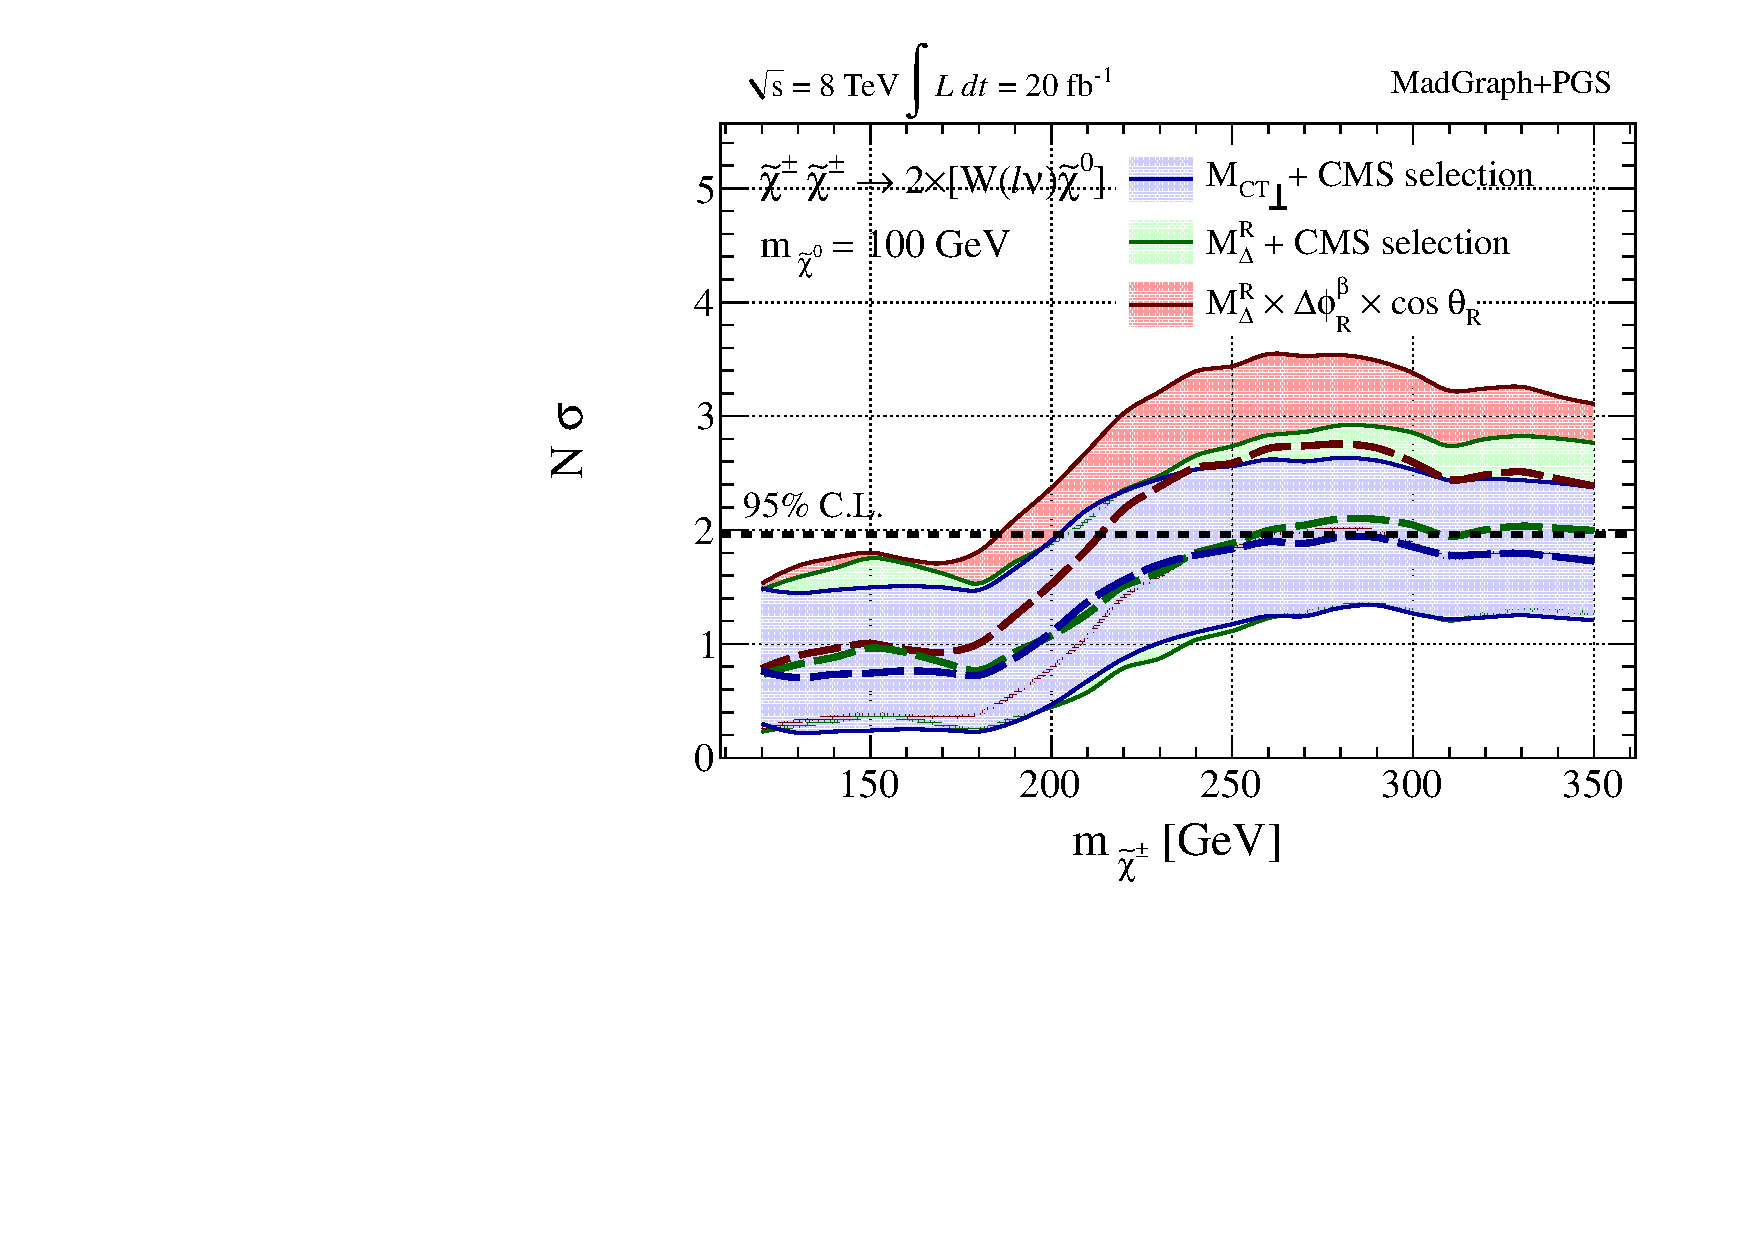
\includegraphics[width=0.40\columnwidth]{fig/sectionV/LIMIT1D_chargino_CMS_MX0100.pdf}
\caption{Expected exclusion limits (in units of $\sigma$) for charginos decaying to neutralinos and leptonic $W$ bosons using 20~fb$^{-1}$ of 8 TeV data, as a function of neutralino mass with 250 GeV charginos (upper and lower left) or as a function of selectron mass with 100 GeV neutralinos (upper and lower right). Expected limits are shown for our multi-dimensional razor analysis (red), and compared to either ATLAS (upper plots) or CMS (lower plots) mass variables and selection criteria. \label{fig:results_chargino_1D_compare}}
\end{figure}
